\documentclass[twoside]{book}

% Packages required by doxygen
\usepackage{fixltx2e}
\usepackage{calc}
\usepackage{doxygen}
\usepackage[export]{adjustbox} % also loads graphicx
\usepackage{graphicx}
\usepackage[utf8]{inputenc}
\usepackage{makeidx}
\usepackage{multicol}
\usepackage{multirow}
\PassOptionsToPackage{warn}{textcomp}
\usepackage{textcomp}
\usepackage[nointegrals]{wasysym}
\usepackage[table]{xcolor}

% Font selection
\usepackage[T1]{fontenc}
\usepackage[scaled=.90]{helvet}
\usepackage{courier}
\usepackage{amssymb}
\usepackage{sectsty}
\renewcommand{\familydefault}{\sfdefault}
\allsectionsfont{%
  \fontseries{bc}\selectfont%
  \color{darkgray}%
}
\renewcommand{\DoxyLabelFont}{%
  \fontseries{bc}\selectfont%
  \color{darkgray}%
}
\newcommand{\+}{\discretionary{\mbox{\scriptsize$\hookleftarrow$}}{}{}}

% Page & text layout
\usepackage{geometry}
\geometry{%
  a4paper,%
  top=2.5cm,%
  bottom=2.5cm,%
  left=2.5cm,%
  right=2.5cm%
}
\tolerance=750
\hfuzz=15pt
\hbadness=750
\setlength{\emergencystretch}{15pt}
\setlength{\parindent}{0cm}
\setlength{\parskip}{3ex plus 2ex minus 2ex}
\makeatletter
\renewcommand{\paragraph}{%
  \@startsection{paragraph}{4}{0ex}{-1.0ex}{1.0ex}{%
    \normalfont\normalsize\bfseries\SS@parafont%
  }%
}
\renewcommand{\subparagraph}{%
  \@startsection{subparagraph}{5}{0ex}{-1.0ex}{1.0ex}{%
    \normalfont\normalsize\bfseries\SS@subparafont%
  }%
}
\makeatother

% Headers & footers
\usepackage{fancyhdr}
\pagestyle{fancyplain}
\fancyhead[LE]{\fancyplain{}{\bfseries\thepage}}
\fancyhead[CE]{\fancyplain{}{}}
\fancyhead[RE]{\fancyplain{}{\bfseries\leftmark}}
\fancyhead[LO]{\fancyplain{}{\bfseries\rightmark}}
\fancyhead[CO]{\fancyplain{}{}}
\fancyhead[RO]{\fancyplain{}{\bfseries\thepage}}
\fancyfoot[LE]{\fancyplain{}{}}
\fancyfoot[CE]{\fancyplain{}{}}
\fancyfoot[RE]{\fancyplain{}{\bfseries\scriptsize Generated by Doxygen }}
\fancyfoot[LO]{\fancyplain{}{\bfseries\scriptsize Generated by Doxygen }}
\fancyfoot[CO]{\fancyplain{}{}}
\fancyfoot[RO]{\fancyplain{}{}}
\renewcommand{\footrulewidth}{0.4pt}
\renewcommand{\chaptermark}[1]{%
  \markboth{#1}{}%
}
\renewcommand{\sectionmark}[1]{%
  \markright{\thesection\ #1}%
}

% Indices & bibliography
\usepackage{natbib}
\usepackage[titles]{tocloft}
\setcounter{tocdepth}{3}
\setcounter{secnumdepth}{5}
\makeindex

% Hyperlinks (required, but should be loaded last)
\usepackage{ifpdf}
\ifpdf
  \usepackage[pdftex,pagebackref=true]{hyperref}
\else
  \usepackage[ps2pdf,pagebackref=true]{hyperref}
\fi
\hypersetup{%
  colorlinks=true,%
  linkcolor=blue,%
  citecolor=blue,%
  unicode%
}

% Custom commands
\newcommand{\clearemptydoublepage}{%
  \newpage{\pagestyle{empty}\cleardoublepage}%
}

\usepackage{caption}
\captionsetup{labelsep=space,justification=centering,font={bf},singlelinecheck=off,skip=4pt,position=top}

%===== C O N T E N T S =====

\begin{document}

% Titlepage & ToC
\hypersetup{pageanchor=false,
             bookmarksnumbered=true,
             pdfencoding=unicode
            }
\pagenumbering{alph}
\begin{titlepage}
\vspace*{7cm}
\begin{center}%
{\Large Lista de Exercícios }\\
\vspace*{1cm}
{\large Generated by Doxygen 1.8.14}\\
\end{center}
\end{titlepage}
\clearemptydoublepage
\pagenumbering{roman}
\tableofcontents
\clearemptydoublepage
\pagenumbering{arabic}
\hypersetup{pageanchor=true}

%--- Begin generated contents ---
\chapter{Hierarchical Index}
\section{Class Hierarchy}
This inheritance list is sorted roughly, but not completely, alphabetically\+:\begin{DoxyCompactList}
\item \contentsline{section}{Account}{\pageref{classAccount}}{}
\item \contentsline{section}{Operation}{\pageref{classOperation}}{}
\item \contentsline{section}{Produto}{\pageref{classProduto}}{}
\begin{DoxyCompactList}
\item \contentsline{section}{Bebida}{\pageref{classBebida}}{}
\item \contentsline{section}{Fruta}{\pageref{classFruta}}{}
\item \contentsline{section}{Roupa}{\pageref{classRoupa}}{}
\end{DoxyCompactList}
\end{DoxyCompactList}

\chapter{Class Index}
\section{Class List}
Here are the classes, structs, unions and interfaces with brief descriptions\+:\begin{DoxyCompactList}
\item\contentsline{section}{\hyperlink{classAccount}{Account} }{\pageref{classAccount}}{}
\item\contentsline{section}{\hyperlink{classBebida}{Bebida} }{\pageref{classBebida}}{}
\item\contentsline{section}{\hyperlink{classFruta}{Fruta} }{\pageref{classFruta}}{}
\item\contentsline{section}{\hyperlink{classOperation}{Operation} }{\pageref{classOperation}}{}
\item\contentsline{section}{\hyperlink{classProduto}{Produto} }{\pageref{classProduto}}{}
\item\contentsline{section}{\hyperlink{classRoupa}{Roupa} }{\pageref{classRoupa}}{}
\end{DoxyCompactList}

\chapter{File Index}
\section{File List}
Here is a list of all documented files with brief descriptions\+:\begin{DoxyCompactList}
\item\contentsline{section}{/home/xsolowingx/\+L\+P1/\+Programas/\+Lista\+Ex/include/questao1/\hyperlink{bebida_8h}{bebida.\+h} \\*Arquivo onde contém as definições da classe \hyperlink{classBebida}{Bebida} }{\pageref{bebida_8h}}{}
\item\contentsline{section}{/home/xsolowingx/\+L\+P1/\+Programas/\+Lista\+Ex/include/questao1/\hyperlink{fruta_8h}{fruta.\+h} \\*Arquivo onde contém as definições da classe \hyperlink{classFruta}{Fruta} }{\pageref{fruta_8h}}{}
\item\contentsline{section}{/home/xsolowingx/\+L\+P1/\+Programas/\+Lista\+Ex/include/questao1/\hyperlink{produto_8h}{produto.\+h} \\*Arquivo onde contém as definições da classe \hyperlink{classProduto}{Produto} }{\pageref{produto_8h}}{}
\item\contentsline{section}{/home/xsolowingx/\+L\+P1/\+Programas/\+Lista\+Ex/include/questao1/\hyperlink{roupa_8h}{roupa.\+h} \\*Arquivo onde contém as definições da classe \hyperlink{classRoupa}{Roupa} }{\pageref{roupa_8h}}{}
\item\contentsline{section}{/home/xsolowingx/\+L\+P1/\+Programas/\+Lista\+Ex/include/questao2/\hyperlink{account_8h}{account.\+h} \\*This file contain the declaration of the class \hyperlink{classAccount}{Account} }{\pageref{account_8h}}{}
\item\contentsline{section}{/home/xsolowingx/\+L\+P1/\+Programas/\+Lista\+Ex/include/questao2/\hyperlink{bank_8h}{bank.\+h} \\*This file contain the declaration of the functions that the bank do }{\pageref{bank_8h}}{}
\item\contentsline{section}{/home/xsolowingx/\+L\+P1/\+Programas/\+Lista\+Ex/include/questao2/\hyperlink{operation_8h}{operation.\+h} \\*This file contain the declaration of the class \hyperlink{classOperation}{Operation} }{\pageref{operation_8h}}{}
\item\contentsline{section}{/home/xsolowingx/\+L\+P1/\+Programas/\+Lista\+Ex/src/questao1/\hyperlink{bebida_8cpp}{bebida.\+cpp} \\*Arquivo onde contém as implementações da classe \hyperlink{classBebida}{Bebida} }{\pageref{bebida_8cpp}}{}
\item\contentsline{section}{/home/xsolowingx/\+L\+P1/\+Programas/\+Lista\+Ex/src/questao1/\hyperlink{fruta_8cpp}{fruta.\+cpp} \\*Arquivo onde contém as implementações da classe \hyperlink{classFruta}{Fruta} }{\pageref{fruta_8cpp}}{}
\item\contentsline{section}{/home/xsolowingx/\+L\+P1/\+Programas/\+Lista\+Ex/src/questao1/\hyperlink{main1_8cpp}{main1.\+cpp} \\*Arquivo principal do programa }{\pageref{main1_8cpp}}{}
\item\contentsline{section}{/home/xsolowingx/\+L\+P1/\+Programas/\+Lista\+Ex/src/questao1/\hyperlink{produto_8cpp}{produto.\+cpp} \\*Arquivo onde contém as implementações da classe \hyperlink{classProduto}{Produto} }{\pageref{produto_8cpp}}{}
\item\contentsline{section}{/home/xsolowingx/\+L\+P1/\+Programas/\+Lista\+Ex/src/questao1/\hyperlink{roupa_8cpp}{roupa.\+cpp} \\*Arquivo onde contém as implementações da classe \hyperlink{classRoupa}{Roupa} }{\pageref{roupa_8cpp}}{}
\item\contentsline{section}{/home/xsolowingx/\+L\+P1/\+Programas/\+Lista\+Ex/src/questao2/\hyperlink{account_8cpp}{account.\+cpp} \\*This file contain the implementation of the class \hyperlink{classAccount}{Account} }{\pageref{account_8cpp}}{}
\item\contentsline{section}{/home/xsolowingx/\+L\+P1/\+Programas/\+Lista\+Ex/src/questao2/\hyperlink{bank_8cpp}{bank.\+cpp} \\*This file contain the implementation of the functions that the bank do }{\pageref{bank_8cpp}}{}
\item\contentsline{section}{/home/xsolowingx/\+L\+P1/\+Programas/\+Lista\+Ex/src/questao2/\hyperlink{main2_8cpp}{main2.\+cpp} \\*This file contain the main program }{\pageref{main2_8cpp}}{}
\item\contentsline{section}{/home/xsolowingx/\+L\+P1/\+Programas/\+Lista\+Ex/src/questao2/\hyperlink{operation_8cpp}{operation.\+cpp} \\*This file contain the implementation of the class \hyperlink{classOperation}{Operation} }{\pageref{operation_8cpp}}{}
\end{DoxyCompactList}

\chapter{Class Documentation}
\hypertarget{classAccount}{}\section{Account Class Reference}
\label{classAccount}\index{Account@{Account}}
\subsection*{Public Member Functions}
\begin{DoxyCompactItemize}
\item 
\mbox{\Hypertarget{classAccount_a3869a254c393605babed6f3027fc4b79}\label{classAccount_a3869a254c393605babed6f3027fc4b79}} 
{\bfseries Account} (std\+::string \+\_\+agency, std\+::string \+\_\+number, Type\+Account \+\_\+type\+\_\+account, std\+::string \+\_\+password)
\item 
\mbox{\Hypertarget{classAccount_a82632554b95fe252b4f245739bac8d27}\label{classAccount_a82632554b95fe252b4f245739bac8d27}} 
void {\bfseries set\+Limit} (float \+\_\+limit)
\item 
\mbox{\Hypertarget{classAccount_a1f341640de88d628019530b70b1b9431}\label{classAccount_a1f341640de88d628019530b70b1b9431}} 
void {\bfseries set\+Balance} (float \+\_\+balance)
\item 
\mbox{\Hypertarget{classAccount_a48071ecda1ec46aebce5f8379d346528}\label{classAccount_a48071ecda1ec46aebce5f8379d346528}} 
void {\bfseries add\+Operation} (\hyperlink{classOperation}{Operation} $\ast$\+\_\+operations)
\item 
\mbox{\Hypertarget{classAccount_a732975b513ba454378ca1c91942b23ba}\label{classAccount_a732975b513ba454378ca1c91942b23ba}} 
std\+::vector$<$ \hyperlink{classOperation}{Operation} $\ast$ $>$\+::iterator {\bfseries operations\+B\+E\+G\+IN} ()
\item 
\mbox{\Hypertarget{classAccount_a3f499b3a04b88756d0a2542898155218}\label{classAccount_a3f499b3a04b88756d0a2542898155218}} 
std\+::vector$<$ \hyperlink{classOperation}{Operation} $\ast$ $>$\+::iterator {\bfseries operations\+E\+ND} ()
\item 
\mbox{\Hypertarget{classAccount_a6da81204de964b2097469ee5ff904603}\label{classAccount_a6da81204de964b2097469ee5ff904603}} 
std\+::string {\bfseries get\+Agency} ()
\item 
\mbox{\Hypertarget{classAccount_a829e1a323877c6d99cfa327f4515a2c4}\label{classAccount_a829e1a323877c6d99cfa327f4515a2c4}} 
std\+::string {\bfseries get\+Number} ()
\item 
\mbox{\Hypertarget{classAccount_aa810a2202edd55c76649fb66d3348416}\label{classAccount_aa810a2202edd55c76649fb66d3348416}} 
std\+::string {\bfseries get\+Password} ()
\item 
\mbox{\Hypertarget{classAccount_a579bd8d93fa3bcbf78dc9cba275eb269}\label{classAccount_a579bd8d93fa3bcbf78dc9cba275eb269}} 
float {\bfseries get\+Limit} ()
\item 
\mbox{\Hypertarget{classAccount_a70d66b5495190c8eacff6ff08eee36df}\label{classAccount_a70d66b5495190c8eacff6ff08eee36df}} 
Type\+Account {\bfseries get\+Type\+\_\+account} ()
\item 
\mbox{\Hypertarget{classAccount_a6a55c17b886dce3a59b18bb746ba4301}\label{classAccount_a6a55c17b886dce3a59b18bb746ba4301}} 
float {\bfseries get\+Balance} ()
\item 
\mbox{\Hypertarget{classAccount_ac285f3e2c3e893cbece0c100cbe49659}\label{classAccount_ac285f3e2c3e893cbece0c100cbe49659}} 
bool {\bfseries operator==} (\hyperlink{classAccount}{Account} \&acc)
\end{DoxyCompactItemize}
\subsection*{Static Public Member Functions}
\begin{DoxyCompactItemize}
\item 
\mbox{\Hypertarget{classAccount_ab709beb9e2fc1233aacb62ffcbcd2144}\label{classAccount_ab709beb9e2fc1233aacb62ffcbcd2144}} 
static int {\bfseries get\+Total\+Accounts} ()
\end{DoxyCompactItemize}
\subsection*{Static Public Attributes}
\begin{DoxyCompactItemize}
\item 
\mbox{\Hypertarget{classAccount_a302696062a8878a4bd013249dd5bc823}\label{classAccount_a302696062a8878a4bd013249dd5bc823}} 
static int {\bfseries Total\+Accounts} = 0
\end{DoxyCompactItemize}
\subsection*{Friends}
\begin{DoxyCompactItemize}
\item 
\mbox{\Hypertarget{classAccount_ad6ea1ae381a91af7074fbfab1374cd03}\label{classAccount_ad6ea1ae381a91af7074fbfab1374cd03}} 
std\+::ostream \& {\bfseries operator$<$$<$} (std\+::ostream \&o, \hyperlink{classAccount}{Account} \&acc)
\end{DoxyCompactItemize}


The documentation for this class was generated from the following files\+:\begin{DoxyCompactItemize}
\item 
/home/xsolowingx/\+L\+P1/\+Programas/\+Lista\+Ex/include/questao2/\hyperlink{account_8h}{account.\+h}\item 
/home/xsolowingx/\+L\+P1/\+Programas/\+Lista\+Ex/src/questao2/\hyperlink{account_8cpp}{account.\+cpp}\end{DoxyCompactItemize}

\hypertarget{classBebida}{}\section{Bebida Class Reference}
\label{classBebida}\index{Bebida@{Bebida}}
Inheritance diagram for Bebida\+:\begin{figure}[H]
\begin{center}
\leavevmode
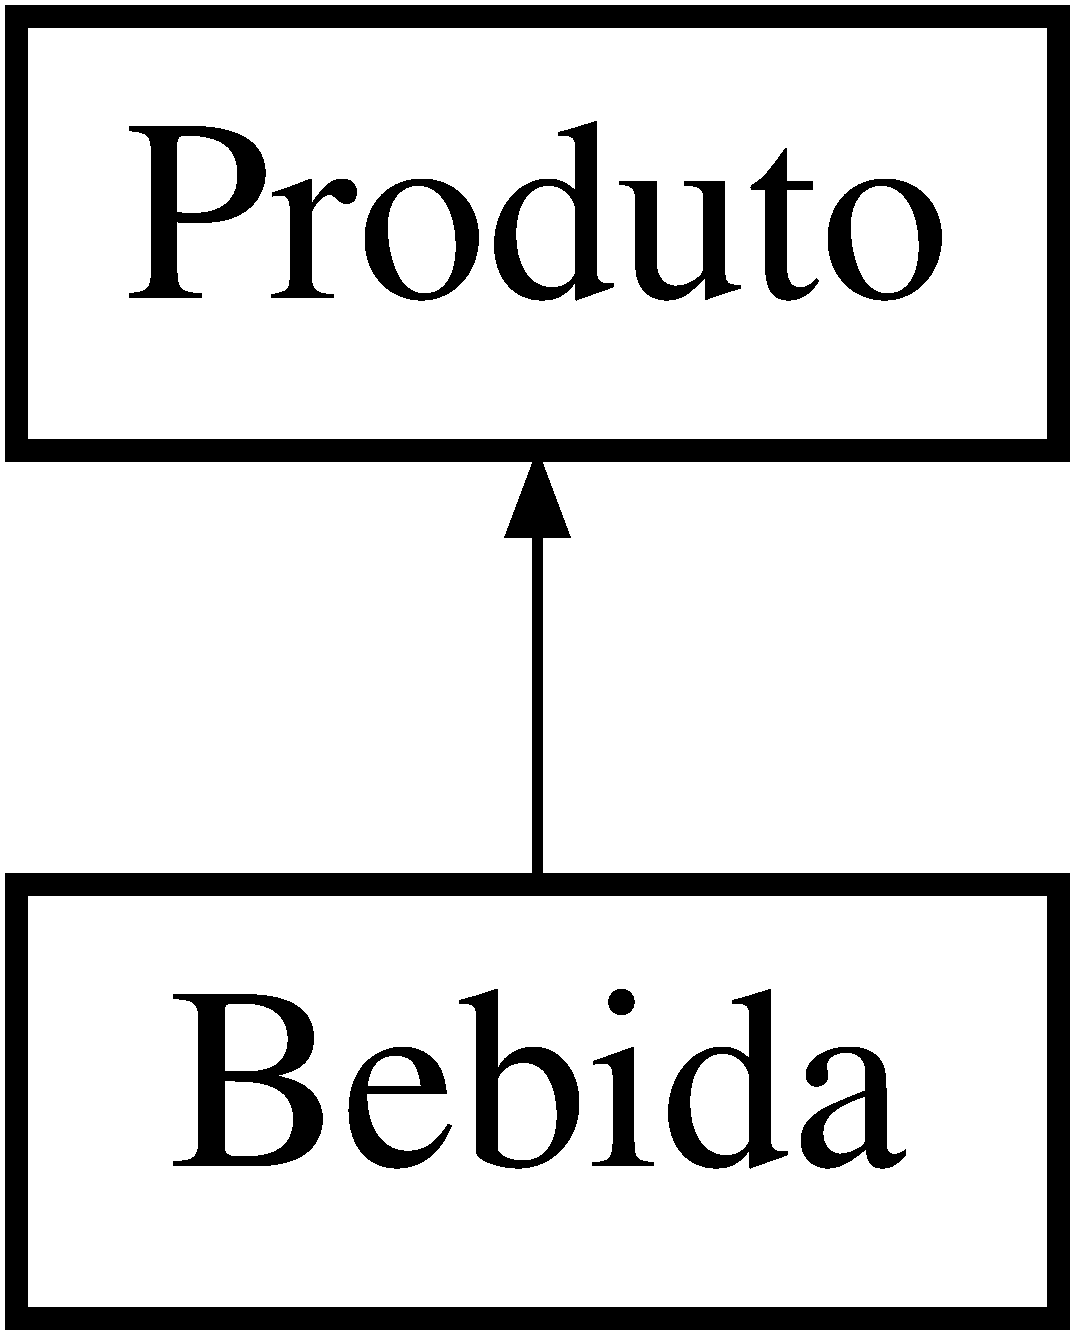
\includegraphics[height=2.000000cm]{classBebida}
\end{center}
\end{figure}
\subsection*{Public Member Functions}
\begin{DoxyCompactItemize}
\item 
\mbox{\Hypertarget{classBebida_a59a7ebfcb70cb79fabf6d57e9a7dc237}\label{classBebida_a59a7ebfcb70cb79fabf6d57e9a7dc237}} 
{\bfseries Bebida} (std\+::string \+\_\+codigo, std\+::string \+\_\+descricao, double \+\_\+preco, std\+::string \+\_\+teor\+\_\+alcoolico)
\item 
\mbox{\Hypertarget{classBebida_ad50198899597b2d2afb290e9d538dbef}\label{classBebida_ad50198899597b2d2afb290e9d538dbef}} 
std\+::string {\bfseries get\+Teor\+Alcoolico} () const
\item 
\mbox{\Hypertarget{classBebida_aa88a16e72690278cb8cc88c1f98c8b14}\label{classBebida_aa88a16e72690278cb8cc88c1f98c8b14}} 
void {\bfseries set\+Teor\+Alcoolico} (std\+::string teor\+\_\+alcoolico\+\_\+da\+\_\+bebida)
\end{DoxyCompactItemize}
\subsection*{Additional Inherited Members}


The documentation for this class was generated from the following files\+:\begin{DoxyCompactItemize}
\item 
/home/xsolowingx/\+L\+P1/\+Programas/\+Lista\+Ex/include/questao1/\hyperlink{bebida_8h}{bebida.\+h}\item 
/home/xsolowingx/\+L\+P1/\+Programas/\+Lista\+Ex/src/questao1/\hyperlink{bebida_8cpp}{bebida.\+cpp}\end{DoxyCompactItemize}

\hypertarget{classConta}{}\section{Conta Class Reference}
\label{classConta}\index{Conta@{Conta}}
Inheritance diagram for Conta\+:\begin{figure}[H]
\begin{center}
\leavevmode
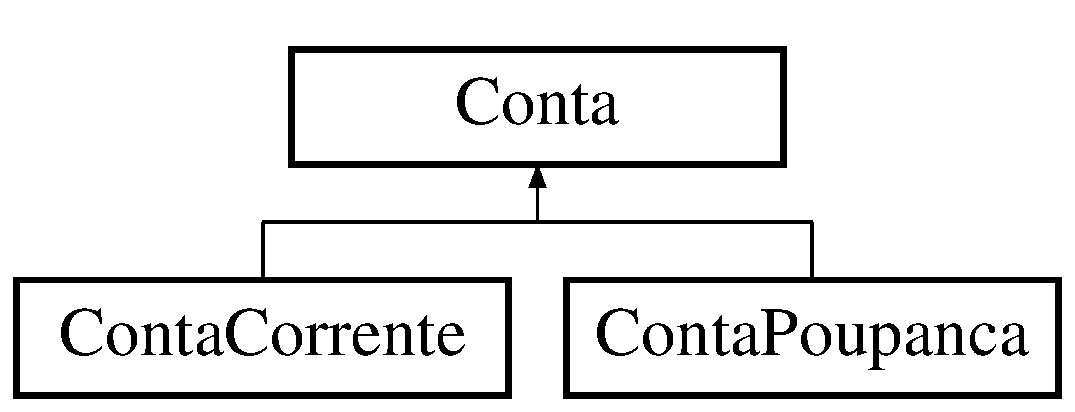
\includegraphics[height=2.000000cm]{classConta}
\end{center}
\end{figure}
\subsection*{Public Member Functions}
\begin{DoxyCompactItemize}
\item 
\mbox{\Hypertarget{classConta_a840bac7d94992024fc14e6c3f37ddf6f}\label{classConta_a840bac7d94992024fc14e6c3f37ddf6f}} 
{\bfseries Conta} (std\+::string \+\_\+agencia, std\+::string \+\_\+numero\+\_\+conta, std\+::string \+\_\+senha, std\+::string \+\_\+titular, Tipo\+Conta \+\_\+tipo\+\_\+da\+\_\+conta)
\item 
\mbox{\Hypertarget{classConta_a36b7092e235e0383387b76dd6d44123f}\label{classConta_a36b7092e235e0383387b76dd6d44123f}} 
void {\bfseries add\+Operacao} (std\+::shared\+\_\+ptr$<$ \hyperlink{classOperacao}{Operacao} $>$ \+\_\+operacao)
\item 
\mbox{\Hypertarget{classConta_a3c15dc4739795232f3bb38bd4ac3f4d9}\label{classConta_a3c15dc4739795232f3bb38bd4ac3f4d9}} 
std\+::vector$<$ std\+::shared\+\_\+ptr$<$ \hyperlink{classOperacao}{Operacao} $>$ $>$\+::iterator {\bfseries operacoes\+B\+E\+G\+IN} ()
\item 
\mbox{\Hypertarget{classConta_a7383512795267f4cd4a2635595c99b12}\label{classConta_a7383512795267f4cd4a2635595c99b12}} 
std\+::vector$<$ std\+::shared\+\_\+ptr$<$ \hyperlink{classOperacao}{Operacao} $>$ $>$\+::iterator {\bfseries operacoes\+E\+ND} ()
\item 
\mbox{\Hypertarget{classConta_a8415b0c8b9571add46e97e31bb9c41a8}\label{classConta_a8415b0c8b9571add46e97e31bb9c41a8}} 
void {\bfseries set\+Saldo} (float \+\_\+saldo\+\_\+)
\item 
\mbox{\Hypertarget{classConta_a64ddf0f8d86ee74e3cf4e1c1c0d934c9}\label{classConta_a64ddf0f8d86ee74e3cf4e1c1c0d934c9}} 
std\+::string {\bfseries get\+Agencia} () const
\item 
\mbox{\Hypertarget{classConta_a1ca2df26b51446e9083d01258abe926a}\label{classConta_a1ca2df26b51446e9083d01258abe926a}} 
std\+::string {\bfseries get\+Numero\+Conta} () const
\item 
\mbox{\Hypertarget{classConta_aace6d48702efd2d146db2e97ba1efba1}\label{classConta_aace6d48702efd2d146db2e97ba1efba1}} 
std\+::string {\bfseries get\+Senha} () const
\item 
\mbox{\Hypertarget{classConta_a59b243246c7b36d84c5d02837df72796}\label{classConta_a59b243246c7b36d84c5d02837df72796}} 
std\+::string {\bfseries get\+Titular} () const
\item 
\mbox{\Hypertarget{classConta_a7d56060e2dcd67d39f87f1b2d51b0742}\label{classConta_a7d56060e2dcd67d39f87f1b2d51b0742}} 
std\+::string {\bfseries get\+TipoC} () const
\item 
\mbox{\Hypertarget{classConta_ade48c55499f84c6c1b261e0c164745e8}\label{classConta_ade48c55499f84c6c1b261e0c164745e8}} 
float {\bfseries get\+Saldo} () const
\item 
\mbox{\Hypertarget{classConta_af2f3d065674824fe8a83c6eccfc99708}\label{classConta_af2f3d065674824fe8a83c6eccfc99708}} 
Tipo\+Conta {\bfseries get\+Tipo\+Conta} () const
\item 
\mbox{\Hypertarget{classConta_a0f9001a717e7f71230a388e726736946}\label{classConta_a0f9001a717e7f71230a388e726736946}} 
void {\bfseries set\+Todos\+Limites\+CP} (int \&LA)
\item 
\mbox{\Hypertarget{classConta_ad48404065aa4c6328bb911e36ddd6a11}\label{classConta_ad48404065aa4c6328bb911e36ddd6a11}} 
void {\bfseries diminui\+Limite} (std\+::string \&tipo)
\item 
\mbox{\Hypertarget{classConta_a3775ce16c33f3ddcb028029c58670231}\label{classConta_a3775ce16c33f3ddcb028029c58670231}} 
virtual float {\bfseries get\+Limite} () const =0
\item 
\mbox{\Hypertarget{classConta_a2bfc21ffd79608809d4f1cc3548619b4}\label{classConta_a2bfc21ffd79608809d4f1cc3548619b4}} 
virtual int {\bfseries get\+Limite\+Saque} () const =0
\item 
\mbox{\Hypertarget{classConta_ae01ea7c06a5e7ffaee8a869a8a358044}\label{classConta_ae01ea7c06a5e7ffaee8a869a8a358044}} 
virtual int {\bfseries get\+Limite\+Extrato} () const =0
\item 
\mbox{\Hypertarget{classConta_afb2847a62f226546b8f21087ef2e5e11}\label{classConta_afb2847a62f226546b8f21087ef2e5e11}} 
virtual int {\bfseries get\+Limite\+Transferencia\+Titular} () const =0
\item 
\mbox{\Hypertarget{classConta_a9e465ff288631a7652321d35a197e3e5}\label{classConta_a9e465ff288631a7652321d35a197e3e5}} 
bool {\bfseries operator==} (\hyperlink{classConta}{Conta} \&c) const
\end{DoxyCompactItemize}
\subsection*{Static Public Member Functions}
\begin{DoxyCompactItemize}
\item 
\mbox{\Hypertarget{classConta_abf3c5cda8fa7689e60a2e803e20f1b9c}\label{classConta_abf3c5cda8fa7689e60a2e803e20f1b9c}} 
static int {\bfseries get\+Total\+Contas} ()
\end{DoxyCompactItemize}
\subsection*{Static Public Attributes}
\begin{DoxyCompactItemize}
\item 
\mbox{\Hypertarget{classConta_aebf38c8207570f4e4a01661e2850c2c5}\label{classConta_aebf38c8207570f4e4a01661e2850c2c5}} 
static int {\bfseries total\+Contas} = 0
\end{DoxyCompactItemize}
\subsection*{Protected Attributes}
\begin{DoxyCompactItemize}
\item 
\mbox{\Hypertarget{classConta_a0e0e322eae287419ad9a6a240a1a6da7}\label{classConta_a0e0e322eae287419ad9a6a240a1a6da7}} 
std\+::string {\bfseries agencia}
\item 
\mbox{\Hypertarget{classConta_aac9f75d95a6dceb3d187ffa5bc57f199}\label{classConta_aac9f75d95a6dceb3d187ffa5bc57f199}} 
std\+::string {\bfseries numero\+\_\+conta}
\item 
\mbox{\Hypertarget{classConta_ab121ceb2a3148f85dfc70835482a00eb}\label{classConta_ab121ceb2a3148f85dfc70835482a00eb}} 
std\+::string {\bfseries senha}
\item 
\mbox{\Hypertarget{classConta_adf5a21c3c3e8bcd7e2eddfa45b8309e8}\label{classConta_adf5a21c3c3e8bcd7e2eddfa45b8309e8}} 
std\+::string {\bfseries titular}
\item 
\mbox{\Hypertarget{classConta_a64e730e4e21e877cdf0f15b9120c31cb}\label{classConta_a64e730e4e21e877cdf0f15b9120c31cb}} 
std\+::vector$<$ std\+::shared\+\_\+ptr$<$ \hyperlink{classOperacao}{Operacao} $>$ $>$ {\bfseries operacoes}
\item 
\mbox{\Hypertarget{classConta_afd9e6b0e5caca532e4d1ee39cf788d5b}\label{classConta_afd9e6b0e5caca532e4d1ee39cf788d5b}} 
Tipo\+Conta {\bfseries tipo\+\_\+da\+\_\+conta}
\item 
\mbox{\Hypertarget{classConta_a0eedc43379194352bb6d117e2d58b9ad}\label{classConta_a0eedc43379194352bb6d117e2d58b9ad}} 
float {\bfseries saldo}
\end{DoxyCompactItemize}
\subsection*{Friends}
\begin{DoxyCompactItemize}
\item 
\mbox{\Hypertarget{classConta_a476b15f634990aaa823054868f60b976}\label{classConta_a476b15f634990aaa823054868f60b976}} 
std\+::ostream \& {\bfseries operator$<$$<$} (std\+::ostream \&o, \hyperlink{classConta}{Conta} const \&c)
\end{DoxyCompactItemize}


The documentation for this class was generated from the following files\+:\begin{DoxyCompactItemize}
\item 
/home/xsolowingx/\+L\+P1/\+Programas/\+Lista\+Ex/include/questao3/\hyperlink{conta_8h}{conta.\+h}\item 
/home/xsolowingx/\+L\+P1/\+Programas/\+Lista\+Ex/src/questao3/\hyperlink{conta_8cpp}{conta.\+cpp}\end{DoxyCompactItemize}

\hypertarget{classContaCorrente}{}\section{Conta\+Corrente Class Reference}
\label{classContaCorrente}\index{Conta\+Corrente@{Conta\+Corrente}}
Inheritance diagram for Conta\+Corrente\+:\begin{figure}[H]
\begin{center}
\leavevmode
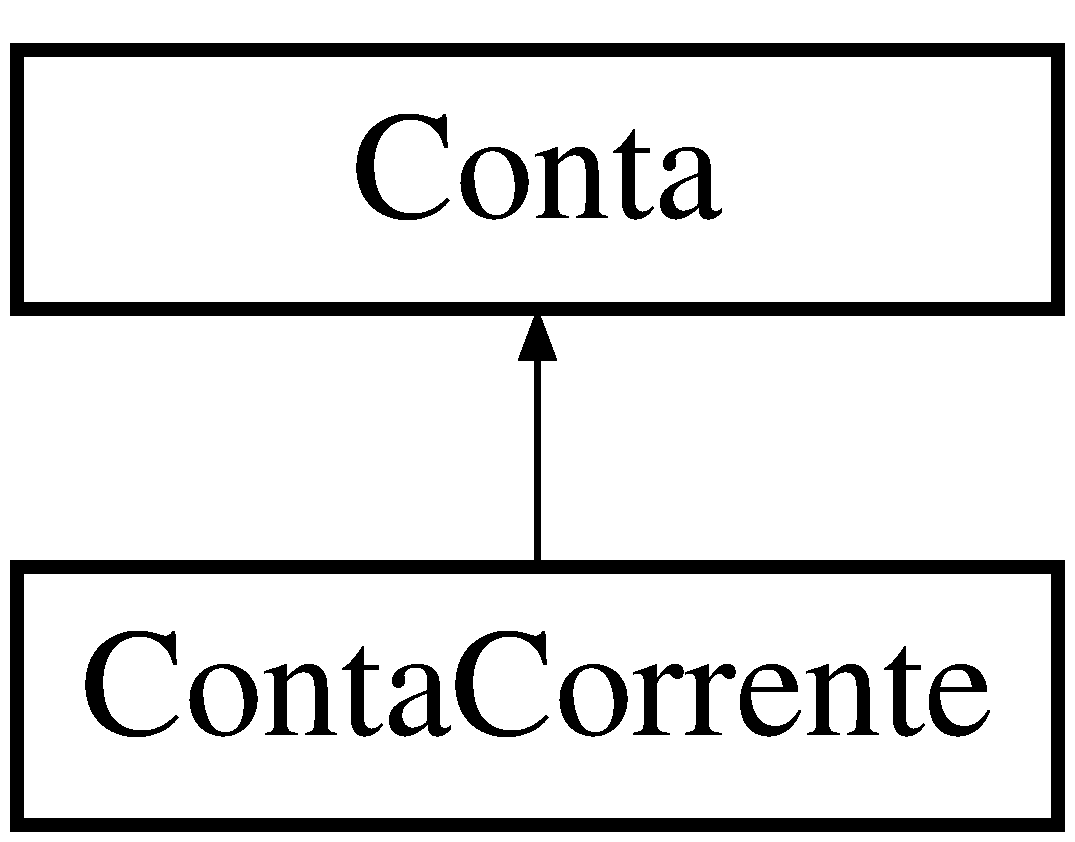
\includegraphics[height=2.000000cm]{classContaCorrente}
\end{center}
\end{figure}
\subsection*{Public Member Functions}
\begin{DoxyCompactItemize}
\item 
\mbox{\Hypertarget{classContaCorrente_a4966c27e501949d89d57661d7e15b500}\label{classContaCorrente_a4966c27e501949d89d57661d7e15b500}} 
{\bfseries Conta\+Corrente} (std\+::string \+\_\+agencia, std\+::string \+\_\+numero\+\_\+conta, std\+::string \+\_\+senha, std\+::string \+\_\+titular, Tipo\+Conta \+\_\+tipo\+\_\+da\+\_\+conta)
\item 
\mbox{\Hypertarget{classContaCorrente_a922280174c72536f9c7fab57e211e979}\label{classContaCorrente_a922280174c72536f9c7fab57e211e979}} 
float {\bfseries get\+Limite} () const
\item 
\mbox{\Hypertarget{classContaCorrente_ae408fca46febd65fc87bc875510b3414}\label{classContaCorrente_ae408fca46febd65fc87bc875510b3414}} 
int {\bfseries get\+Limite\+Saque} () const
\item 
\mbox{\Hypertarget{classContaCorrente_a2fa3869476cf98747e6ffd485c620c2e}\label{classContaCorrente_a2fa3869476cf98747e6ffd485c620c2e}} 
int {\bfseries get\+Limite\+Extrato} () const
\item 
\mbox{\Hypertarget{classContaCorrente_a9e19f26b74af3203c6bce445f863decf}\label{classContaCorrente_a9e19f26b74af3203c6bce445f863decf}} 
int {\bfseries get\+Limite\+Transferencia\+Titular} () const
\end{DoxyCompactItemize}
\subsection*{Additional Inherited Members}


The documentation for this class was generated from the following files\+:\begin{DoxyCompactItemize}
\item 
/home/xsolowingx/\+L\+P1/\+Programas/\+Lista\+Ex/include/questao3/\hyperlink{contaCorrente_8h}{conta\+Corrente.\+h}\item 
/home/xsolowingx/\+L\+P1/\+Programas/\+Lista\+Ex/src/questao3/\hyperlink{contaCorrente_8cpp}{conta\+Corrente.\+cpp}\end{DoxyCompactItemize}

\hypertarget{classContaPoupanca}{}\section{Conta\+Poupanca Class Reference}
\label{classContaPoupanca}\index{Conta\+Poupanca@{Conta\+Poupanca}}
Inheritance diagram for Conta\+Poupanca\+:\begin{figure}[H]
\begin{center}
\leavevmode
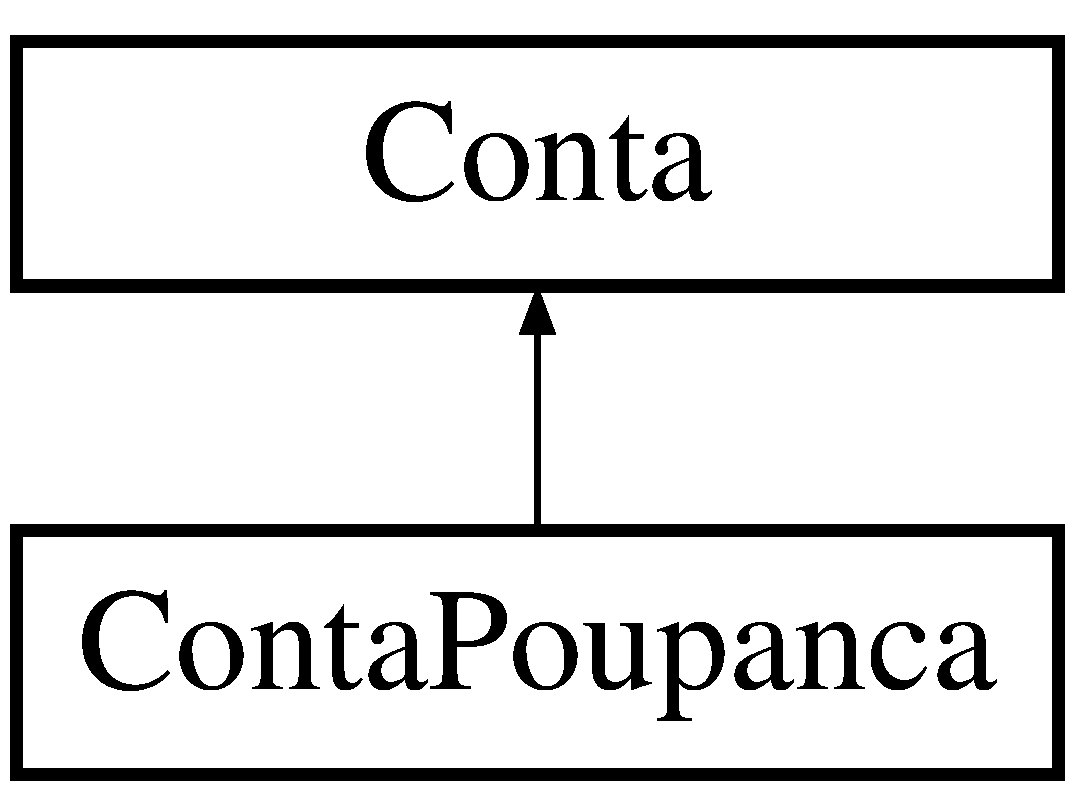
\includegraphics[height=2.000000cm]{classContaPoupanca}
\end{center}
\end{figure}
\subsection*{Public Member Functions}
\begin{DoxyCompactItemize}
\item 
\mbox{\Hypertarget{classContaPoupanca_a80d4955cdfe5d9ab14fe067ef2e92236}\label{classContaPoupanca_a80d4955cdfe5d9ab14fe067ef2e92236}} 
{\bfseries Conta\+Poupanca} (std\+::string \+\_\+agencia, std\+::string \+\_\+numero\+\_\+conta, std\+::string \+\_\+senha, std\+::string \+\_\+titular, Tipo\+Conta \+\_\+tipo\+\_\+da\+\_\+conta)
\item 
\mbox{\Hypertarget{classContaPoupanca_a33a69fa8c291ba8509fd643c0a55445c}\label{classContaPoupanca_a33a69fa8c291ba8509fd643c0a55445c}} 
void {\bfseries set\+Todos\+Limites\+C\+PD} (int \&LA)
\item 
\mbox{\Hypertarget{classContaPoupanca_aa56dd906d9b47915b65038b0968d0289}\label{classContaPoupanca_aa56dd906d9b47915b65038b0968d0289}} 
void {\bfseries diminui\+LimiteD} (std\+::string \&tipo)
\item 
\mbox{\Hypertarget{classContaPoupanca_a8ec6d2bf7c6304ca896b032603dedc6a}\label{classContaPoupanca_a8ec6d2bf7c6304ca896b032603dedc6a}} 
int {\bfseries get\+Limite\+Saque} () const
\item 
\mbox{\Hypertarget{classContaPoupanca_a273c0e693efe41ccb44e1acbf1ce6728}\label{classContaPoupanca_a273c0e693efe41ccb44e1acbf1ce6728}} 
int {\bfseries get\+Limite\+Extrato} () const
\item 
\mbox{\Hypertarget{classContaPoupanca_a0c4ba4e299a936ba30bf3bdad0fe199b}\label{classContaPoupanca_a0c4ba4e299a936ba30bf3bdad0fe199b}} 
int {\bfseries get\+Limite\+Transferencia\+Titular} () const
\item 
\mbox{\Hypertarget{classContaPoupanca_a53c74e9136c70e1c015d3cec18c3ed9c}\label{classContaPoupanca_a53c74e9136c70e1c015d3cec18c3ed9c}} 
float {\bfseries get\+Limite} () const
\end{DoxyCompactItemize}
\subsection*{Additional Inherited Members}


The documentation for this class was generated from the following files\+:\begin{DoxyCompactItemize}
\item 
/home/xsolowingx/\+L\+P1/\+Programas/\+Lista\+Ex/include/questao3/\hyperlink{contaPoupanca_8h}{conta\+Poupanca.\+h}\item 
/home/xsolowingx/\+L\+P1/\+Programas/\+Lista\+Ex/src/questao3/\hyperlink{contaPoupanca_8cpp}{conta\+Poupanca.\+cpp}\end{DoxyCompactItemize}

\hypertarget{classFruta}{}\section{Fruta Class Reference}
\label{classFruta}\index{Fruta@{Fruta}}
Inheritance diagram for Fruta\+:\begin{figure}[H]
\begin{center}
\leavevmode
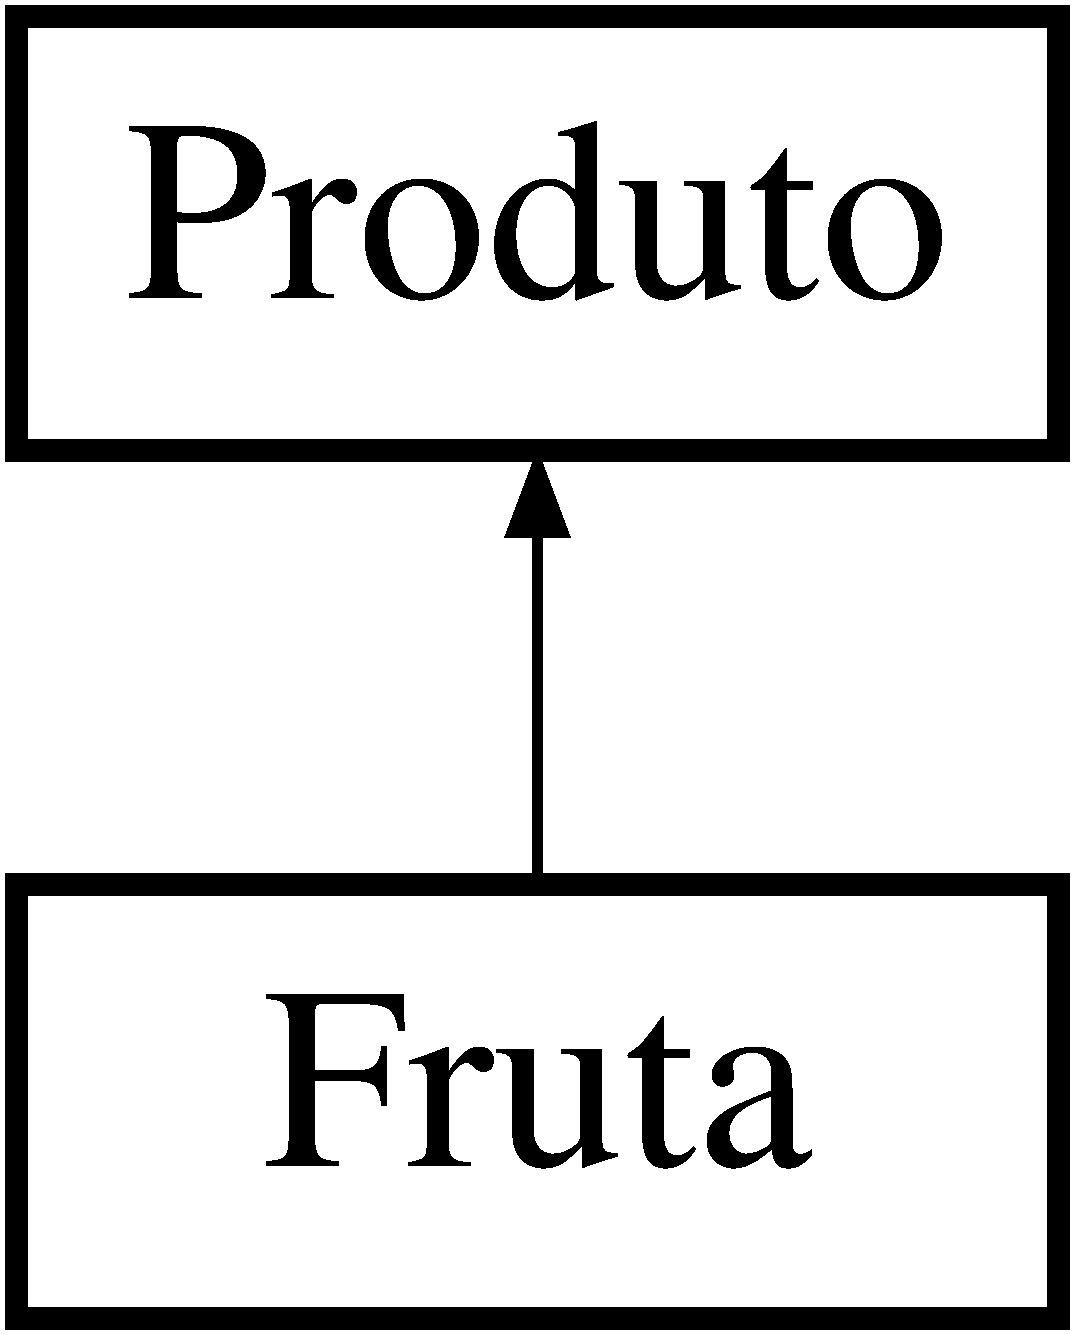
\includegraphics[height=2.000000cm]{classFruta}
\end{center}
\end{figure}
\subsection*{Public Member Functions}
\begin{DoxyCompactItemize}
\item 
\mbox{\Hypertarget{classFruta_a2bf2dce96b7094cf9fbb8b90d3516842}\label{classFruta_a2bf2dce96b7094cf9fbb8b90d3516842}} 
{\bfseries Fruta} (std\+::string \+\_\+codigo, std\+::string \+\_\+descricao, double \+\_\+preco, std\+::string \+\_\+data, double \+\_\+validade)
\item 
\mbox{\Hypertarget{classFruta_a60347bd8c61fe2face180ccde8fa93d0}\label{classFruta_a60347bd8c61fe2face180ccde8fa93d0}} 
std\+::string {\bfseries get\+Data\+Lote} () const
\item 
\mbox{\Hypertarget{classFruta_a6508a7308482bb7c43a21fd187485242}\label{classFruta_a6508a7308482bb7c43a21fd187485242}} 
double {\bfseries get\+Validade} () const
\item 
\mbox{\Hypertarget{classFruta_aa6cc01d8af01018e0a90b91e91884c13}\label{classFruta_aa6cc01d8af01018e0a90b91e91884c13}} 
void {\bfseries set\+Data\+Lote} (std\+::string \+\_\+data)
\item 
\mbox{\Hypertarget{classFruta_a11112ce25fe41bf796a487d818b16406}\label{classFruta_a11112ce25fe41bf796a487d818b16406}} 
void {\bfseries set\+Validade} (double \+\_\+validade)
\end{DoxyCompactItemize}
\subsection*{Additional Inherited Members}


The documentation for this class was generated from the following files\+:\begin{DoxyCompactItemize}
\item 
/home/xsolowingx/\+L\+P1/\+Programas/\+Lista\+Ex/include/questao1/\hyperlink{fruta_8h}{fruta.\+h}\item 
/home/xsolowingx/\+L\+P1/\+Programas/\+Lista\+Ex/src/questao1/\hyperlink{fruta_8cpp}{fruta.\+cpp}\end{DoxyCompactItemize}

\hypertarget{classOperacao}{}\section{Operacao Class Reference}
\label{classOperacao}\index{Operacao@{Operacao}}
\subsection*{Public Member Functions}
\begin{DoxyCompactItemize}
\item 
\mbox{\Hypertarget{classOperacao_ae4468beed2e7eb355cc953fc8cb8d1ca}\label{classOperacao_ae4468beed2e7eb355cc953fc8cb8d1ca}} 
{\bfseries Operacao} (std\+::string \+\_\+descricao, Tipo\+Operacao \+\_\+tipo\+\_\+operacao, float \+\_\+valor)
\item 
\mbox{\Hypertarget{classOperacao_a35f87140b7cfb4630d0fb990fca04a93}\label{classOperacao_a35f87140b7cfb4630d0fb990fca04a93}} 
std\+::string {\bfseries get\+Descricao} () const
\item 
\mbox{\Hypertarget{classOperacao_a722ca5d89c46ca6ac74ba09a384b3373}\label{classOperacao_a722ca5d89c46ca6ac74ba09a384b3373}} 
Tipo\+Operacao {\bfseries get\+Tipo\+\_\+operacao} () const
\item 
\mbox{\Hypertarget{classOperacao_aec71392c25861acd3c7eee0cf9a740f7}\label{classOperacao_aec71392c25861acd3c7eee0cf9a740f7}} 
float {\bfseries get\+Valor} () const
\end{DoxyCompactItemize}
\subsection*{Friends}
\begin{DoxyCompactItemize}
\item 
\mbox{\Hypertarget{classOperacao_ac2839c47d817b524aa30e0ee1e32fe87}\label{classOperacao_ac2839c47d817b524aa30e0ee1e32fe87}} 
std\+::ostream \& {\bfseries operator$<$$<$} (std\+::ostream \&o, \hyperlink{classOperacao}{Operacao} const \&op)
\end{DoxyCompactItemize}


The documentation for this class was generated from the following files\+:\begin{DoxyCompactItemize}
\item 
/home/xsolowingx/\+L\+P1/\+Programas/\+Lista\+Ex/include/questao3/\hyperlink{operacao_8h}{operacao.\+h}\item 
/home/xsolowingx/\+L\+P1/\+Programas/\+Lista\+Ex/src/questao3/\hyperlink{operacao_8cpp}{operacao.\+cpp}\end{DoxyCompactItemize}

\hypertarget{classOperation}{}\section{Operation Class Reference}
\label{classOperation}\index{Operation@{Operation}}
\subsection*{Public Member Functions}
\begin{DoxyCompactItemize}
\item 
\mbox{\Hypertarget{classOperation_a2b8a8d86b297a45c1a677cc3d7af9174}\label{classOperation_a2b8a8d86b297a45c1a677cc3d7af9174}} 
{\bfseries Operation} (std\+::string \+\_\+description, Type\+Operation \+\_\+type\+\_\+operation, float \+\_\+value)
\item 
\mbox{\Hypertarget{classOperation_a9b2a4bda36bca3b14c5b76e8f6a47d93}\label{classOperation_a9b2a4bda36bca3b14c5b76e8f6a47d93}} 
float {\bfseries get\+Value} ()
\item 
\mbox{\Hypertarget{classOperation_a6ab35e3b17952fcb981d7b8768b15f3d}\label{classOperation_a6ab35e3b17952fcb981d7b8768b15f3d}} 
std\+::string {\bfseries get\+Description} ()
\item 
\mbox{\Hypertarget{classOperation_a7fc75204f0374b316b16f410398dd62b}\label{classOperation_a7fc75204f0374b316b16f410398dd62b}} 
Type\+Operation {\bfseries get\+Type\+\_\+operation} ()
\end{DoxyCompactItemize}
\subsection*{Friends}
\begin{DoxyCompactItemize}
\item 
\mbox{\Hypertarget{classOperation_a2595e2d474930011c8adb05ccfd16ea4}\label{classOperation_a2595e2d474930011c8adb05ccfd16ea4}} 
std\+::ostream \& {\bfseries operator$<$$<$} (std\+::ostream \&o, \hyperlink{classOperation}{Operation} operation)
\end{DoxyCompactItemize}


The documentation for this class was generated from the following files\+:\begin{DoxyCompactItemize}
\item 
/home/xsolowingx/\+L\+P1/\+Programas/\+Lista\+Ex/include/questao2/\hyperlink{operation_8h}{operation.\+h}\item 
/home/xsolowingx/\+L\+P1/\+Programas/\+Lista\+Ex/src/questao2/\hyperlink{operation_8cpp}{operation.\+cpp}\end{DoxyCompactItemize}

\hypertarget{classProduto}{}\section{Produto Class Reference}
\label{classProduto}\index{Produto@{Produto}}
Inheritance diagram for Produto\+:\begin{figure}[H]
\begin{center}
\leavevmode
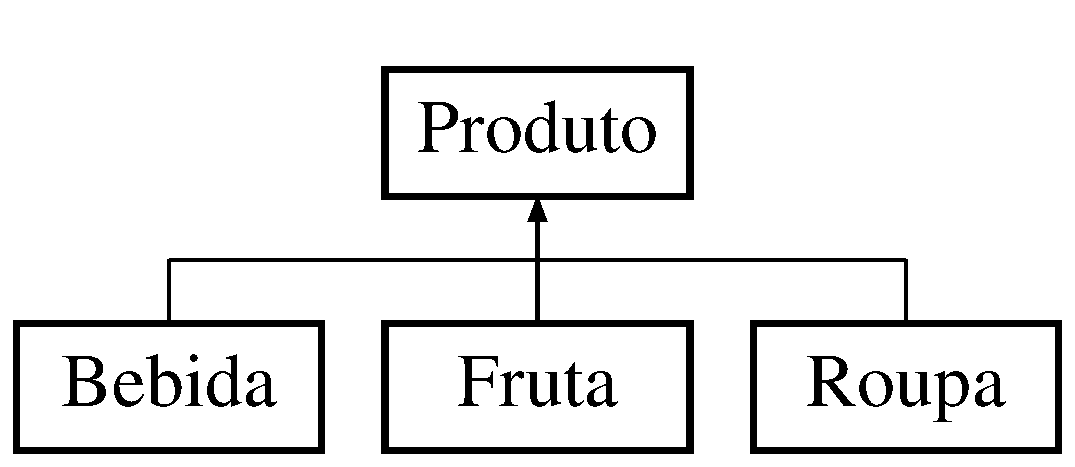
\includegraphics[height=2.000000cm]{classProduto}
\end{center}
\end{figure}
\subsection*{Public Member Functions}
\begin{DoxyCompactItemize}
\item 
\mbox{\Hypertarget{classProduto_a12dc783d4f1e016d1eefea0b3f83a6b0}\label{classProduto_a12dc783d4f1e016d1eefea0b3f83a6b0}} 
{\bfseries Produto} (std\+::string \+\_\+codigo, std\+::string \+\_\+descricao, double \+\_\+preco)
\item 
\mbox{\Hypertarget{classProduto_afe2d2b5330ac2a4be858141aa7ec1e96}\label{classProduto_afe2d2b5330ac2a4be858141aa7ec1e96}} 
std\+::string {\bfseries get\+Cod\+Barras} () const
\item 
\mbox{\Hypertarget{classProduto_acf6b619f58c3e69a3ecaa0946cc83699}\label{classProduto_acf6b619f58c3e69a3ecaa0946cc83699}} 
std\+::string {\bfseries get\+Descricao} () const
\item 
\mbox{\Hypertarget{classProduto_ace1d384192a7f2cfc7768afa6b7fcbf5}\label{classProduto_ace1d384192a7f2cfc7768afa6b7fcbf5}} 
double {\bfseries get\+Preco} () const
\item 
\mbox{\Hypertarget{classProduto_a8f8e7d58e53d3f175bc41b2481dbf477}\label{classProduto_a8f8e7d58e53d3f175bc41b2481dbf477}} 
void {\bfseries set\+Cod\+Barras} (std\+::string \+\_\+codigo)
\item 
\mbox{\Hypertarget{classProduto_a35b8ac377821ca2197becf75e1063509}\label{classProduto_a35b8ac377821ca2197becf75e1063509}} 
void {\bfseries set\+Descricao} (std\+::string \+\_\+descricao)
\item 
\mbox{\Hypertarget{classProduto_a207ec4b3438d376227ca3053a14669cf}\label{classProduto_a207ec4b3438d376227ca3053a14669cf}} 
void {\bfseries set\+Preco} (double \+\_\+preco)
\item 
\mbox{\Hypertarget{classProduto_ae5330ecb2af5add388ff14500f2fe67a}\label{classProduto_ae5330ecb2af5add388ff14500f2fe67a}} 
{\bfseries operator double} ()
\item 
\mbox{\Hypertarget{classProduto_a2495b539fbd1efa333867c29dce4af7a}\label{classProduto_a2495b539fbd1efa333867c29dce4af7a}} 
bool {\bfseries operator==} (\hyperlink{classProduto}{Produto} const \&p)
\item 
\mbox{\Hypertarget{classProduto_a4100739cbf6a9d7a23c4c4299a1192be}\label{classProduto_a4100739cbf6a9d7a23c4c4299a1192be}} 
double {\bfseries operator+} (\hyperlink{classProduto}{Produto} const \&p)
\item 
\mbox{\Hypertarget{classProduto_a442790572afe412a6e5ef32c0b81c1ce}\label{classProduto_a442790572afe412a6e5ef32c0b81c1ce}} 
double {\bfseries operator-\/} (\hyperlink{classProduto}{Produto} const \&p)
\end{DoxyCompactItemize}
\subsection*{Protected Attributes}
\begin{DoxyCompactItemize}
\item 
\mbox{\Hypertarget{classProduto_a2e772f6b851f2a2c7d7bc6853af7ca83}\label{classProduto_a2e772f6b851f2a2c7d7bc6853af7ca83}} 
std\+::string {\bfseries m\+\_\+cod\+\_\+barras}
\item 
\mbox{\Hypertarget{classProduto_aacf69c2cf01b6040138767a47c1e3f4b}\label{classProduto_aacf69c2cf01b6040138767a47c1e3f4b}} 
std\+::string {\bfseries m\+\_\+descricao}
\item 
\mbox{\Hypertarget{classProduto_af4f68aad97167802a1dca2b8ddb188eb}\label{classProduto_af4f68aad97167802a1dca2b8ddb188eb}} 
double {\bfseries m\+\_\+preco}
\end{DoxyCompactItemize}
\subsection*{Friends}
\begin{DoxyCompactItemize}
\item 
\mbox{\Hypertarget{classProduto_a3f8bbab15d5b8943ac04af1bc6eec1bf}\label{classProduto_a3f8bbab15d5b8943ac04af1bc6eec1bf}} 
std\+::ostream \& {\bfseries operator$<$$<$} (std\+::ostream \&o, \hyperlink{classProduto}{Produto} const \&p)
\end{DoxyCompactItemize}


The documentation for this class was generated from the following files\+:\begin{DoxyCompactItemize}
\item 
/home/xsolowingx/\+L\+P1/\+Programas/\+Lista\+Ex/include/questao1/\hyperlink{produto_8h}{produto.\+h}\item 
/home/xsolowingx/\+L\+P1/\+Programas/\+Lista\+Ex/src/questao1/\hyperlink{produto_8cpp}{produto.\+cpp}\end{DoxyCompactItemize}

\hypertarget{classRoupa}{}\section{Roupa Class Reference}
\label{classRoupa}\index{Roupa@{Roupa}}
Inheritance diagram for Roupa\+:\begin{figure}[H]
\begin{center}
\leavevmode
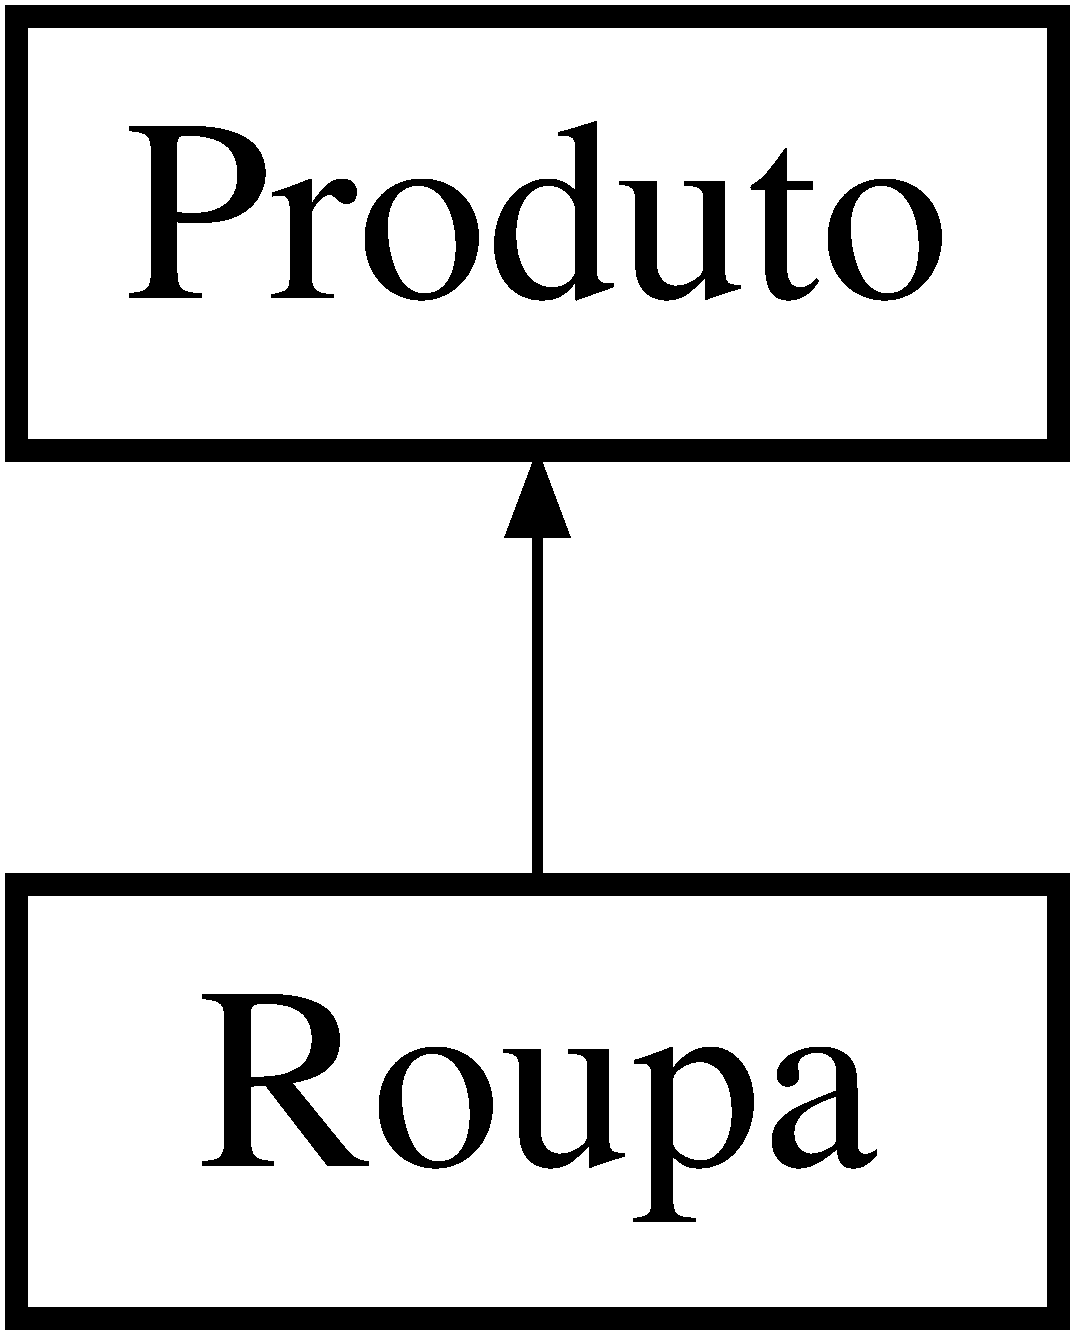
\includegraphics[height=2.000000cm]{classRoupa}
\end{center}
\end{figure}
\subsection*{Public Member Functions}
\begin{DoxyCompactItemize}
\item 
\mbox{\Hypertarget{classRoupa_a6deaef1b59d73712322ef805a7585140}\label{classRoupa_a6deaef1b59d73712322ef805a7585140}} 
{\bfseries Roupa} (std\+::string \+\_\+codigo, std\+::string \+\_\+descricao, double \+\_\+preco, std\+::string \+\_\+marca, char \+\_\+sexo, std\+::string \+\_\+tamanho)
\item 
\mbox{\Hypertarget{classRoupa_a2bf426a4019f698230095573a0bf089c}\label{classRoupa_a2bf426a4019f698230095573a0bf089c}} 
std\+::string {\bfseries get\+Marca} () const
\item 
\mbox{\Hypertarget{classRoupa_a4881596b2683965fe9c689c71383b1c2}\label{classRoupa_a4881596b2683965fe9c689c71383b1c2}} 
char {\bfseries get\+Sexo} () const
\item 
\mbox{\Hypertarget{classRoupa_af49bdcfcefc426815a89f77b4f2083a6}\label{classRoupa_af49bdcfcefc426815a89f77b4f2083a6}} 
std\+::string {\bfseries get\+Tamanho} () const
\item 
\mbox{\Hypertarget{classRoupa_a779827a9b55aa33229413fa441f45ab7}\label{classRoupa_a779827a9b55aa33229413fa441f45ab7}} 
void {\bfseries set\+Marca} (std\+::string \+\_\+marca)
\item 
\mbox{\Hypertarget{classRoupa_a40e8636ee6b49b145924b155dbd57690}\label{classRoupa_a40e8636ee6b49b145924b155dbd57690}} 
void {\bfseries set\+Sexo} (char \+\_\+sexo)
\item 
\mbox{\Hypertarget{classRoupa_ab5541947bc4fde1925422eab8cc6b190}\label{classRoupa_ab5541947bc4fde1925422eab8cc6b190}} 
void {\bfseries set\+Tamanho} (std\+::string \+\_\+tamanho)
\end{DoxyCompactItemize}
\subsection*{Additional Inherited Members}


The documentation for this class was generated from the following files\+:\begin{DoxyCompactItemize}
\item 
/home/xsolowingx/\+L\+P1/\+Programas/\+Lista\+Ex/include/questao1/\hyperlink{roupa_8h}{roupa.\+h}\item 
/home/xsolowingx/\+L\+P1/\+Programas/\+Lista\+Ex/src/questao1/\hyperlink{roupa_8cpp}{roupa.\+cpp}\end{DoxyCompactItemize}

\chapter{File Documentation}
\hypertarget{bebida_8h}{}\section{/home/xsolowingx/\+L\+P1/\+Programas/\+Lista\+Ex/include/questao1/bebida.h File Reference}
\label{bebida_8h}\index{/home/xsolowingx/\+L\+P1/\+Programas/\+Lista\+Ex/include/questao1/bebida.\+h@{/home/xsolowingx/\+L\+P1/\+Programas/\+Lista\+Ex/include/questao1/bebida.\+h}}


arquivo onde contém as definições da classe \hyperlink{classBebida}{Bebida}.  


{\ttfamily \#include \char`\"{}produto.\+h\char`\"{}}\newline
\subsection*{Classes}
\begin{DoxyCompactItemize}
\item 
class \hyperlink{classBebida}{Bebida}
\end{DoxyCompactItemize}


\subsection{Detailed Description}
arquivo onde contém as definições da classe \hyperlink{classBebida}{Bebida}. 

\begin{DoxySince}{Since}
10/10/2017
\end{DoxySince}
\begin{DoxyAuthor}{Author}
Matheus de Jesus Leandro de Medeiros 
\end{DoxyAuthor}
\begin{DoxyDate}{Date}
13/10/2017 
\end{DoxyDate}

\hypertarget{fruta_8h}{}\section{/home/xsolowingx/\+L\+P1/\+Programas/\+Lista\+Ex/include/questao1/fruta.h File Reference}
\label{fruta_8h}\index{/home/xsolowingx/\+L\+P1/\+Programas/\+Lista\+Ex/include/questao1/fruta.\+h@{/home/xsolowingx/\+L\+P1/\+Programas/\+Lista\+Ex/include/questao1/fruta.\+h}}


arquivo onde contém as definições da classe \hyperlink{classFruta}{Fruta}.  


{\ttfamily \#include \char`\"{}produto.\+h\char`\"{}}\newline
\subsection*{Classes}
\begin{DoxyCompactItemize}
\item 
class \hyperlink{classFruta}{Fruta}
\end{DoxyCompactItemize}


\subsection{Detailed Description}
arquivo onde contém as definições da classe \hyperlink{classFruta}{Fruta}. 

\begin{DoxySince}{Since}
10/10/2017
\end{DoxySince}
\begin{DoxyAuthor}{Author}
Matheus de Jesus Leandro de Medeiros 
\end{DoxyAuthor}
\begin{DoxyDate}{Date}
13/10/2017 
\end{DoxyDate}

\hypertarget{produto_8h}{}\section{/home/xsolowingx/\+L\+P1/\+Programas/\+Lista\+Ex/include/questao1/produto.h File Reference}
\label{produto_8h}\index{/home/xsolowingx/\+L\+P1/\+Programas/\+Lista\+Ex/include/questao1/produto.\+h@{/home/xsolowingx/\+L\+P1/\+Programas/\+Lista\+Ex/include/questao1/produto.\+h}}


arquivo onde contém as definições da classe \hyperlink{classProduto}{Produto}.  


{\ttfamily \#include $<$iostream$>$}\newline
{\ttfamily \#include $<$string$>$}\newline
{\ttfamily \#include $<$ostream$>$}\newline
\subsection*{Classes}
\begin{DoxyCompactItemize}
\item 
class \hyperlink{classProduto}{Produto}
\end{DoxyCompactItemize}


\subsection{Detailed Description}
arquivo onde contém as definições da classe \hyperlink{classProduto}{Produto}. 

\begin{DoxySince}{Since}
10/10/2017
\end{DoxySince}
\begin{DoxyAuthor}{Author}
Matheus de Jesus Leandro de Medeiros 
\end{DoxyAuthor}
\begin{DoxyDate}{Date}
13/10/2017 
\end{DoxyDate}

\hypertarget{roupa_8h}{}\section{/home/xsolowingx/\+L\+P1/\+Programas/\+Lista\+Ex/include/questao1/roupa.h File Reference}
\label{roupa_8h}\index{/home/xsolowingx/\+L\+P1/\+Programas/\+Lista\+Ex/include/questao1/roupa.\+h@{/home/xsolowingx/\+L\+P1/\+Programas/\+Lista\+Ex/include/questao1/roupa.\+h}}


arquivo onde contém as definições da classe \hyperlink{classRoupa}{Roupa}.  


{\ttfamily \#include \char`\"{}produto.\+h\char`\"{}}\newline
\subsection*{Classes}
\begin{DoxyCompactItemize}
\item 
class \hyperlink{classRoupa}{Roupa}
\end{DoxyCompactItemize}


\subsection{Detailed Description}
arquivo onde contém as definições da classe \hyperlink{classRoupa}{Roupa}. 

\begin{DoxySince}{Since}
10/10/2017
\end{DoxySince}
\begin{DoxyAuthor}{Author}
Matheus de Jesus Leandro de Medeiros 
\end{DoxyAuthor}
\begin{DoxyDate}{Date}
13/10/2017 
\end{DoxyDate}

\hypertarget{account_8h}{}\section{/home/xsolowingx/\+L\+P1/\+Programas/\+Lista\+Ex/include/questao2/account.h File Reference}
\label{account_8h}\index{/home/xsolowingx/\+L\+P1/\+Programas/\+Lista\+Ex/include/questao2/account.\+h@{/home/xsolowingx/\+L\+P1/\+Programas/\+Lista\+Ex/include/questao2/account.\+h}}


this file contain the declaration of the class \hyperlink{classAccount}{Account}.  


{\ttfamily \#include \char`\"{}operation.\+h\char`\"{}}\newline
{\ttfamily \#include $<$vector$>$}\newline
{\ttfamily \#include $<$ostream$>$}\newline
\subsection*{Classes}
\begin{DoxyCompactItemize}
\item 
class \hyperlink{classAccount}{Account}
\end{DoxyCompactItemize}
\subsection*{Typedefs}
\begin{DoxyCompactItemize}
\item 
\mbox{\Hypertarget{account_8h_ac538cb1d78a97bf08ed363aa329f073e}\label{account_8h_ac538cb1d78a97bf08ed363aa329f073e}} 
typedef enum str\+\_\+especial {\bfseries Type\+Account}
\item 
\mbox{\Hypertarget{account_8h_acca0bdcdec201de464a2ca59f907c7f8}\label{account_8h_acca0bdcdec201de464a2ca59f907c7f8}} 
typedef enum str\+\_\+type {\bfseries Type\+Helper}
\end{DoxyCompactItemize}
\subsection*{Enumerations}
\begin{DoxyCompactItemize}
\item 
\mbox{\Hypertarget{account_8h_a941bf0c85766ea4c0cd6b3805f63161c}\label{account_8h_a941bf0c85766ea4c0cd6b3805f63161c}} 
enum {\bfseries str\+\_\+especial} \{ \newline
{\bfseries Special}, 
{\bfseries Normal}, 
{\bfseries Especial}, 
{\bfseries Normal}, 
\newline
{\bfseries Poupanca}
 \}
\item 
\mbox{\Hypertarget{account_8h_a89ed1cc1b672afaa8805b00b4650a523}\label{account_8h_a89ed1cc1b672afaa8805b00b4650a523}} 
enum {\bfseries str\+\_\+type} \{ {\bfseries Correct}, 
{\bfseries Wrong}
 \}
\end{DoxyCompactItemize}


\subsection{Detailed Description}
this file contain the declaration of the class \hyperlink{classAccount}{Account}. 

\begin{DoxySince}{Since}
09/17/2017
\end{DoxySince}
\begin{DoxyAuthor}{Author}
Matheus de Jesus Leandro de Medeiros 
\end{DoxyAuthor}
\begin{DoxyDate}{Date}
09/22/2017 
\end{DoxyDate}

\hypertarget{bank_8h}{}\section{/home/xsolowingx/\+L\+P1/\+Programas/\+Lista\+Ex/include/questao2/bank.h File Reference}
\label{bank_8h}\index{/home/xsolowingx/\+L\+P1/\+Programas/\+Lista\+Ex/include/questao2/bank.\+h@{/home/xsolowingx/\+L\+P1/\+Programas/\+Lista\+Ex/include/questao2/bank.\+h}}


this file contain the declaration of the functions that the bank do.  


{\ttfamily \#include \char`\"{}account.\+h\char`\"{}}\newline
\subsection*{Functions}
\begin{DoxyCompactItemize}
\item 
\mbox{\Hypertarget{bank_8h_a07871231951a0016e975d7b6437da5a1}\label{bank_8h_a07871231951a0016e975d7b6437da5a1}} 
void {\bfseries create\+Account} (std\+::vector$<$ \hyperlink{classAccount}{Account} $\ast$$>$ \&accounts)
\item 
\mbox{\Hypertarget{bank_8h_a80387282660ea054c6a08a2dcc217c66}\label{bank_8h_a80387282660ea054c6a08a2dcc217c66}} 
void {\bfseries deposit} (std\+::vector$<$ \hyperlink{classAccount}{Account} $\ast$$>$ \&accounts)
\item 
\mbox{\Hypertarget{bank_8h_aac0fab1780b1fc907d71f45ffc4c106a}\label{bank_8h_aac0fab1780b1fc907d71f45ffc4c106a}} 
void {\bfseries withdraw} (std\+::vector$<$ \hyperlink{classAccount}{Account} $\ast$$>$ \&accounts)
\item 
\mbox{\Hypertarget{bank_8h_acfa72e05415de6230d000e95b9b14d3b}\label{bank_8h_acfa72e05415de6230d000e95b9b14d3b}} 
void {\bfseries delete\+Account} (std\+::vector$<$ \hyperlink{classAccount}{Account} $\ast$$>$ \&accounts)
\item 
\mbox{\Hypertarget{bank_8h_adc5db9f43e2adb5b4672711d0e27a39a}\label{bank_8h_adc5db9f43e2adb5b4672711d0e27a39a}} 
void {\bfseries list\+Accounts} (std\+::vector$<$ \hyperlink{classAccount}{Account} $\ast$$>$ \&accounts)
\item 
\mbox{\Hypertarget{bank_8h_aa3b48bfe56b69e1bf2e1efdfb756890a}\label{bank_8h_aa3b48bfe56b69e1bf2e1efdfb756890a}} 
void {\bfseries transfer} (std\+::vector$<$ \hyperlink{classAccount}{Account} $\ast$$>$ \&accounts)
\item 
\mbox{\Hypertarget{bank_8h_abbf200c777d7eabafdd4dc7217150a3f}\label{bank_8h_abbf200c777d7eabafdd4dc7217150a3f}} 
void {\bfseries see\+Balance} (std\+::vector$<$ \hyperlink{classAccount}{Account} $\ast$$>$ \&accounts)
\item 
\mbox{\Hypertarget{bank_8h_ab14172549ecb01ff668007d311a0cafd}\label{bank_8h_ab14172549ecb01ff668007d311a0cafd}} 
void {\bfseries Bank\+Statement} (std\+::vector$<$ \hyperlink{classAccount}{Account} $\ast$$>$ \&accounts)
\item 
\mbox{\Hypertarget{bank_8h_a01c328a75e8cf7087d6036d780901e30}\label{bank_8h_a01c328a75e8cf7087d6036d780901e30}} 
bool {\bfseries verify\+Account} (std\+::string \&\+\_\+agency\+\_\+, std\+::string \&\+\_\+number\+\_\+, std\+::vector$<$ \hyperlink{classAccount}{Account} $\ast$$>$ \&accounts)
\item 
\mbox{\Hypertarget{bank_8h_a35f75289f5c16348a049be04eaa9228d}\label{bank_8h_a35f75289f5c16348a049be04eaa9228d}} 
bool {\bfseries verify\+Yes\+\_\+\+No} ()
\item 
\mbox{\Hypertarget{bank_8h_a014efcbd3b224059c11e194e86da29de}\label{bank_8h_a014efcbd3b224059c11e194e86da29de}} 
void {\bfseries verify\+Password} (\hyperlink{classAccount}{Account} \&acc)
\item 
\mbox{\Hypertarget{bank_8h_acea0b2bca6b72de82e8004a13ee032f0}\label{bank_8h_acea0b2bca6b72de82e8004a13ee032f0}} 
void {\bfseries begin\+Message} ()
\item 
\mbox{\Hypertarget{bank_8h_a2a0e843767aeea4f433a28b9c54f573a}\label{bank_8h_a2a0e843767aeea4f433a28b9c54f573a}} 
void {\bfseries menu} ()
\item 
\mbox{\Hypertarget{bank_8h_a9079ce99dfe463edff71ca373917a035}\label{bank_8h_a9079ce99dfe463edff71ca373917a035}} 
void {\bfseries input\+Number} (std\+::string \&number)
\item 
\mbox{\Hypertarget{bank_8h_ad558c4d8d5ab3a546e1d0ca4cd24e80d}\label{bank_8h_ad558c4d8d5ab3a546e1d0ca4cd24e80d}} 
void {\bfseries input\+NumberF} (std\+::string \&number)
\end{DoxyCompactItemize}


\subsection{Detailed Description}
this file contain the declaration of the functions that the bank do. 

\begin{DoxySince}{Since}
09/17/2017
\end{DoxySince}
\begin{DoxyAuthor}{Author}
Matheus de Jesus Leandro de Medeiros 
\end{DoxyAuthor}
\begin{DoxyDate}{Date}
09/22/2017 
\end{DoxyDate}

\hypertarget{operation_8h}{}\section{/home/xsolowingx/\+L\+P1/\+Programas/\+Lista\+Ex/include/questao2/operation.h File Reference}
\label{operation_8h}\index{/home/xsolowingx/\+L\+P1/\+Programas/\+Lista\+Ex/include/questao2/operation.\+h@{/home/xsolowingx/\+L\+P1/\+Programas/\+Lista\+Ex/include/questao2/operation.\+h}}


this file contain the declaration of the class \hyperlink{classOperation}{Operation}.  


{\ttfamily \#include $<$string$>$}\newline
{\ttfamily \#include $<$ostream$>$}\newline
\subsection*{Classes}
\begin{DoxyCompactItemize}
\item 
class \hyperlink{classOperation}{Operation}
\end{DoxyCompactItemize}
\subsection*{Typedefs}
\begin{DoxyCompactItemize}
\item 
\mbox{\Hypertarget{operation_8h_a0a29cbbcd19cc6fa5e219bc5ea150993}\label{operation_8h_a0a29cbbcd19cc6fa5e219bc5ea150993}} 
typedef enum str\+Type {\bfseries Type\+Operation}
\end{DoxyCompactItemize}
\subsection*{Enumerations}
\begin{DoxyCompactItemize}
\item 
\mbox{\Hypertarget{operation_8h_af0c207f7ab3948266f3d486f44928790}\label{operation_8h_af0c207f7ab3948266f3d486f44928790}} 
enum {\bfseries str\+Type} \{ {\bfseries Debit}, 
{\bfseries Credit}, 
{\bfseries Debito}, 
{\bfseries Credito}
 \}
\end{DoxyCompactItemize}


\subsection{Detailed Description}
this file contain the declaration of the class \hyperlink{classOperation}{Operation}. 

\begin{DoxySince}{Since}
09/17/2017
\end{DoxySince}
\begin{DoxyAuthor}{Author}
Matheus de Jesus Leandro de Medeiros 
\end{DoxyAuthor}
\begin{DoxyDate}{Date}
09/22/2017 
\end{DoxyDate}

\hypertarget{banco_8h}{}\section{/home/xsolowingx/\+L\+P1/\+Programas/\+Lista\+Ex/include/questao3/banco.h File Reference}
\label{banco_8h}\index{/home/xsolowingx/\+L\+P1/\+Programas/\+Lista\+Ex/include/questao3/banco.\+h@{/home/xsolowingx/\+L\+P1/\+Programas/\+Lista\+Ex/include/questao3/banco.\+h}}


arquivo onde contém as definições das funções do banco.  


{\ttfamily \#include \char`\"{}conta.\+h\char`\"{}}\newline
\subsection*{Functions}
\begin{DoxyCompactItemize}
\item 
\mbox{\Hypertarget{banco_8h_aef9c58b5f7bea8101eaed6b2dea1a096}\label{banco_8h_aef9c58b5f7bea8101eaed6b2dea1a096}} 
void {\bfseries criar\+Conta} (std\+::vector$<$ std\+::shared\+\_\+ptr$<$ \hyperlink{classConta}{Conta} $>$$>$ \&contas)
\item 
\mbox{\Hypertarget{banco_8h_a597eb5a16a25823e1f7c7f642dc47fd2}\label{banco_8h_a597eb5a16a25823e1f7c7f642dc47fd2}} 
void {\bfseries deposito} (std\+::vector$<$ std\+::shared\+\_\+ptr$<$ \hyperlink{classConta}{Conta} $>$$>$ \&contas)
\item 
\mbox{\Hypertarget{banco_8h_a9cd5a8ec566ea871270cf65bedda319e}\label{banco_8h_a9cd5a8ec566ea871270cf65bedda319e}} 
void {\bfseries saque} (std\+::vector$<$ std\+::shared\+\_\+ptr$<$ \hyperlink{classConta}{Conta} $>$$>$ \&contas)
\item 
\mbox{\Hypertarget{banco_8h_a2f050ea778a4f4c4c028ed59c2c28ca0}\label{banco_8h_a2f050ea778a4f4c4c028ed59c2c28ca0}} 
void {\bfseries deletar\+Conta} (std\+::vector$<$ std\+::shared\+\_\+ptr$<$ \hyperlink{classConta}{Conta} $>$$>$ \&contas)
\item 
\mbox{\Hypertarget{banco_8h_a2ad81220e3c7b53ced55bfd76fb255b2}\label{banco_8h_a2ad81220e3c7b53ced55bfd76fb255b2}} 
void {\bfseries listar\+Contas} (std\+::vector$<$ std\+::shared\+\_\+ptr$<$ \hyperlink{classConta}{Conta} $>$$>$ \&contas)
\item 
\mbox{\Hypertarget{banco_8h_a0cdf5cac1e3ebcd5da625327caec5282}\label{banco_8h_a0cdf5cac1e3ebcd5da625327caec5282}} 
void {\bfseries transferencia} (std\+::vector$<$ std\+::shared\+\_\+ptr$<$ \hyperlink{classConta}{Conta} $>$$>$ \&contas)
\item 
\mbox{\Hypertarget{banco_8h_a7e814b976f0e940568e477eb3842af47}\label{banco_8h_a7e814b976f0e940568e477eb3842af47}} 
void {\bfseries ve\+Saldo} (std\+::vector$<$ std\+::shared\+\_\+ptr$<$ \hyperlink{classConta}{Conta} $>$$>$ \&contas)
\item 
\mbox{\Hypertarget{banco_8h_a80b39cc6a7b4c560a17f6eb38c093731}\label{banco_8h_a80b39cc6a7b4c560a17f6eb38c093731}} 
void {\bfseries extrato\+Bancario} (std\+::vector$<$ std\+::shared\+\_\+ptr$<$ \hyperlink{classConta}{Conta} $>$$>$ \&contas)
\item 
\mbox{\Hypertarget{banco_8h_a8013403a874bef279e02989ee41548e2}\label{banco_8h_a8013403a874bef279e02989ee41548e2}} 
bool {\bfseries verifica\+Conta} (std\+::string \&\+\_\+agencia\+\_\+, std\+::string \&\+\_\+numero\+\_\+conta\+\_\+, std\+::vector$<$ std\+::shared\+\_\+ptr$<$ \hyperlink{classConta}{Conta} $>$$>$ \&contas)
\item 
\mbox{\Hypertarget{banco_8h_ac67e012e8ecfa66947183de841dd14ae}\label{banco_8h_ac67e012e8ecfa66947183de841dd14ae}} 
bool {\bfseries verifica\+Sim\+\_\+\+Nao} ()
\item 
\mbox{\Hypertarget{banco_8h_aef1152c51b001637006df0ab72bbcf50}\label{banco_8h_aef1152c51b001637006df0ab72bbcf50}} 
void {\bfseries verifica\+Senha} (\hyperlink{classConta}{Conta} \&contaP)
\item 
\mbox{\Hypertarget{banco_8h_ad2611953204db49693c98283ab6f0d80}\label{banco_8h_ad2611953204db49693c98283ab6f0d80}} 
void {\bfseries mensagem\+Inicio} ()
\item 
\mbox{\Hypertarget{banco_8h_a2a0e843767aeea4f433a28b9c54f573a}\label{banco_8h_a2a0e843767aeea4f433a28b9c54f573a}} 
void {\bfseries menu} ()
\item 
\mbox{\Hypertarget{banco_8h_aad17b10ee307aba3b8de3671efc738c2}\label{banco_8h_aad17b10ee307aba3b8de3671efc738c2}} 
void {\bfseries input\+NumberI} (std\+::string \&number)
\item 
\mbox{\Hypertarget{banco_8h_ad558c4d8d5ab3a546e1d0ca4cd24e80d}\label{banco_8h_ad558c4d8d5ab3a546e1d0ca4cd24e80d}} 
void {\bfseries input\+NumberF} (std\+::string \&number)
\item 
\mbox{\Hypertarget{banco_8h_a7c1c37c23cc36fb230564971c889692b}\label{banco_8h_a7c1c37c23cc36fb230564971c889692b}} 
void {\bfseries input\+Name} (std\+::string \&name)
\end{DoxyCompactItemize}


\subsection{Detailed Description}
arquivo onde contém as definições das funções do banco. 

\begin{DoxySince}{Since}
15/10/2017
\end{DoxySince}
\begin{DoxyAuthor}{Author}
Matheus de Jesus Leandro de Medeiros 
\end{DoxyAuthor}
\begin{DoxyDate}{Date}
23/10/2017 
\end{DoxyDate}

\hypertarget{conta_8h}{}\section{/home/xsolowingx/\+L\+P1/\+Programas/\+Lista\+Ex/include/questao3/conta.h File Reference}
\label{conta_8h}\index{/home/xsolowingx/\+L\+P1/\+Programas/\+Lista\+Ex/include/questao3/conta.\+h@{/home/xsolowingx/\+L\+P1/\+Programas/\+Lista\+Ex/include/questao3/conta.\+h}}


esse arquivo contém as definições da classe \hyperlink{classConta}{Conta}.  


{\ttfamily \#include $<$string$>$}\newline
{\ttfamily \#include $<$vector$>$}\newline
{\ttfamily \#include $<$ostream$>$}\newline
{\ttfamily \#include $<$memory$>$}\newline
{\ttfamily \#include \char`\"{}operacao.\+h\char`\"{}}\newline
\subsection*{Classes}
\begin{DoxyCompactItemize}
\item 
class \hyperlink{classConta}{Conta}
\end{DoxyCompactItemize}
\subsection*{Typedefs}
\begin{DoxyCompactItemize}
\item 
\mbox{\Hypertarget{conta_8h_a18c09b198bc9b63b37d7fed7c9c7365b}\label{conta_8h_a18c09b198bc9b63b37d7fed7c9c7365b}} 
typedef enum str\+\_\+especial {\bfseries Tipo\+Conta}
\end{DoxyCompactItemize}
\subsection*{Enumerations}
\begin{DoxyCompactItemize}
\item 
\mbox{\Hypertarget{conta_8h_a941bf0c85766ea4c0cd6b3805f63161c}\label{conta_8h_a941bf0c85766ea4c0cd6b3805f63161c}} 
enum {\bfseries str\+\_\+especial} \{ \newline
{\bfseries Special}, 
{\bfseries Normal}, 
{\bfseries Especial}, 
{\bfseries Normal}, 
\newline
{\bfseries Poupanca}
 \}
\end{DoxyCompactItemize}


\subsection{Detailed Description}
esse arquivo contém as definições da classe \hyperlink{classConta}{Conta}. 

\begin{DoxySince}{Since}
15/10/2017
\end{DoxySince}
\begin{DoxyAuthor}{Author}
Matheus de Jesus Leandro de Medeiros 
\end{DoxyAuthor}
\begin{DoxyDate}{Date}
23/10/2017 
\end{DoxyDate}

\hypertarget{contaCorrente_8h}{}\section{/home/xsolowingx/\+L\+P1/\+Programas/\+Lista\+Ex/include/questao3/conta\+Corrente.h File Reference}
\label{contaCorrente_8h}\index{/home/xsolowingx/\+L\+P1/\+Programas/\+Lista\+Ex/include/questao3/conta\+Corrente.\+h@{/home/xsolowingx/\+L\+P1/\+Programas/\+Lista\+Ex/include/questao3/conta\+Corrente.\+h}}


arquivo onde contém as definições da classe \hyperlink{classContaCorrente}{Conta\+Corrente}.  


{\ttfamily \#include \char`\"{}conta.\+h\char`\"{}}\newline
\subsection*{Classes}
\begin{DoxyCompactItemize}
\item 
class \hyperlink{classContaCorrente}{Conta\+Corrente}
\end{DoxyCompactItemize}


\subsection{Detailed Description}
arquivo onde contém as definições da classe \hyperlink{classContaCorrente}{Conta\+Corrente}. 

\begin{DoxySince}{Since}
15/10/2017
\end{DoxySince}
\begin{DoxyAuthor}{Author}
Matheus de Jesus Leandro de Medeiros 
\end{DoxyAuthor}
\begin{DoxyDate}{Date}
23/10/2017 
\end{DoxyDate}

\hypertarget{contaPoupanca_8h}{}\section{/home/xsolowingx/\+L\+P1/\+Programas/\+Lista\+Ex/include/questao3/conta\+Poupanca.h File Reference}
\label{contaPoupanca_8h}\index{/home/xsolowingx/\+L\+P1/\+Programas/\+Lista\+Ex/include/questao3/conta\+Poupanca.\+h@{/home/xsolowingx/\+L\+P1/\+Programas/\+Lista\+Ex/include/questao3/conta\+Poupanca.\+h}}


arquivo onde contém as definições da classe \hyperlink{classContaPoupanca}{Conta\+Poupanca}.  


{\ttfamily \#include \char`\"{}conta.\+h\char`\"{}}\newline
\subsection*{Classes}
\begin{DoxyCompactItemize}
\item 
class \hyperlink{classContaPoupanca}{Conta\+Poupanca}
\end{DoxyCompactItemize}


\subsection{Detailed Description}
arquivo onde contém as definições da classe \hyperlink{classContaPoupanca}{Conta\+Poupanca}. 

\begin{DoxySince}{Since}
15/10/2017
\end{DoxySince}
\begin{DoxyAuthor}{Author}
Matheus de Jesus Leandro de Medeiros 
\end{DoxyAuthor}
\begin{DoxyDate}{Date}
23/10/2017 
\end{DoxyDate}

\hypertarget{operacao_8h}{}\section{/home/xsolowingx/\+L\+P1/\+Programas/\+Lista\+Ex/include/questao3/operacao.h File Reference}
\label{operacao_8h}\index{/home/xsolowingx/\+L\+P1/\+Programas/\+Lista\+Ex/include/questao3/operacao.\+h@{/home/xsolowingx/\+L\+P1/\+Programas/\+Lista\+Ex/include/questao3/operacao.\+h}}


arquivo onde contém as definições da classe \hyperlink{classOperacao}{Operacao}.  


{\ttfamily \#include $<$ostream$>$}\newline
{\ttfamily \#include $<$string$>$}\newline
\subsection*{Classes}
\begin{DoxyCompactItemize}
\item 
class \hyperlink{classOperacao}{Operacao}
\end{DoxyCompactItemize}
\subsection*{Typedefs}
\begin{DoxyCompactItemize}
\item 
\mbox{\Hypertarget{operacao_8h_a277ab88ed8d1ba11b72ba953ed9426ad}\label{operacao_8h_a277ab88ed8d1ba11b72ba953ed9426ad}} 
typedef enum str\+Type {\bfseries Tipo\+Operacao}
\end{DoxyCompactItemize}
\subsection*{Enumerations}
\begin{DoxyCompactItemize}
\item 
\mbox{\Hypertarget{operacao_8h_af0c207f7ab3948266f3d486f44928790}\label{operacao_8h_af0c207f7ab3948266f3d486f44928790}} 
enum {\bfseries str\+Type} \{ {\bfseries Debit}, 
{\bfseries Credit}, 
{\bfseries Debito}, 
{\bfseries Credito}
 \}
\end{DoxyCompactItemize}


\subsection{Detailed Description}
arquivo onde contém as definições da classe \hyperlink{classOperacao}{Operacao}. 

\begin{DoxySince}{Since}
15/10/2017
\end{DoxySince}
\begin{DoxyAuthor}{Author}
Matheus de Jesus Leandro de Medeiros 
\end{DoxyAuthor}
\begin{DoxyDate}{Date}
23/10/2017 
\end{DoxyDate}

\hypertarget{bebida_8cpp}{}\section{/home/xsolowingx/\+L\+P1/\+Programas/\+Lista\+Ex/src/questao1/bebida.cpp File Reference}
\label{bebida_8cpp}\index{/home/xsolowingx/\+L\+P1/\+Programas/\+Lista\+Ex/src/questao1/bebida.\+cpp@{/home/xsolowingx/\+L\+P1/\+Programas/\+Lista\+Ex/src/questao1/bebida.\+cpp}}


arquivo onde contém as implementações da classe \hyperlink{classBebida}{Bebida}.  


{\ttfamily \#include \char`\"{}bebida.\+h\char`\"{}}\newline
{\ttfamily \#include \char`\"{}produto.\+h\char`\"{}}\newline


\subsection{Detailed Description}
arquivo onde contém as implementações da classe \hyperlink{classBebida}{Bebida}. 

\begin{DoxySince}{Since}
10/10/2017
\end{DoxySince}
\begin{DoxyAuthor}{Author}
Matheus de Jesus Leandro de Medeiros 
\end{DoxyAuthor}
\begin{DoxyDate}{Date}
13/10/2017 
\end{DoxyDate}

\hypertarget{fruta_8cpp}{}\section{/home/xsolowingx/\+L\+P1/\+Programas/\+Lista\+Ex/src/questao1/fruta.cpp File Reference}
\label{fruta_8cpp}\index{/home/xsolowingx/\+L\+P1/\+Programas/\+Lista\+Ex/src/questao1/fruta.\+cpp@{/home/xsolowingx/\+L\+P1/\+Programas/\+Lista\+Ex/src/questao1/fruta.\+cpp}}


arquivo onde contém as implementações da classe \hyperlink{classFruta}{Fruta}.  


{\ttfamily \#include $<$iomanip$>$}\newline
{\ttfamily \#include \char`\"{}fruta.\+h\char`\"{}}\newline
{\ttfamily \#include \char`\"{}produto.\+h\char`\"{}}\newline


\subsection{Detailed Description}
arquivo onde contém as implementações da classe \hyperlink{classFruta}{Fruta}. 

\begin{DoxySince}{Since}
10/10/2017
\end{DoxySince}
\begin{DoxyAuthor}{Author}
Matheus de Jesus Leandro de Medeiros 
\end{DoxyAuthor}
\begin{DoxyDate}{Date}
13/10/2017 
\end{DoxyDate}

\hypertarget{main1_8cpp}{}\section{/home/xsolowingx/\+L\+P1/\+Programas/\+Lista\+Ex/src/questao1/main1.cpp File Reference}
\label{main1_8cpp}\index{/home/xsolowingx/\+L\+P1/\+Programas/\+Lista\+Ex/src/questao1/main1.\+cpp@{/home/xsolowingx/\+L\+P1/\+Programas/\+Lista\+Ex/src/questao1/main1.\+cpp}}


arquivo principal do programa.  


{\ttfamily \#include $<$iostream$>$}\newline
{\ttfamily \#include $<$vector$>$}\newline
{\ttfamily \#include $<$memory$>$}\newline
{\ttfamily \#include \char`\"{}produto.\+h\char`\"{}}\newline
{\ttfamily \#include \char`\"{}fruta.\+h\char`\"{}}\newline
{\ttfamily \#include \char`\"{}roupa.\+h\char`\"{}}\newline
{\ttfamily \#include \char`\"{}bebida.\+h\char`\"{}}\newline
\subsection*{Functions}
\begin{DoxyCompactItemize}
\item 
\mbox{\Hypertarget{main1_8cpp_ae66f6b31b5ad750f1fe042a706a4e3d4}\label{main1_8cpp_ae66f6b31b5ad750f1fe042a706a4e3d4}} 
int {\bfseries main} ()
\end{DoxyCompactItemize}


\subsection{Detailed Description}
arquivo principal do programa. 

\begin{DoxySince}{Since}
10/10/2017
\end{DoxySince}
\begin{DoxyAuthor}{Author}
Matheus de Jesus Leandro de Medeiros 
\end{DoxyAuthor}
\begin{DoxyDate}{Date}
13/10/2017 
\end{DoxyDate}

\hypertarget{produto_8cpp}{}\section{/home/xsolowingx/\+L\+P1/\+Programas/\+Lista\+Ex/src/questao1/produto.cpp File Reference}
\label{produto_8cpp}\index{/home/xsolowingx/\+L\+P1/\+Programas/\+Lista\+Ex/src/questao1/produto.\+cpp@{/home/xsolowingx/\+L\+P1/\+Programas/\+Lista\+Ex/src/questao1/produto.\+cpp}}


arquivo onde contém as implementações da classe \hyperlink{classProduto}{Produto}.  


{\ttfamily \#include $<$iostream$>$}\newline
{\ttfamily \#include \char`\"{}produto.\+h\char`\"{}}\newline
\subsection*{Functions}
\begin{DoxyCompactItemize}
\item 
\mbox{\Hypertarget{produto_8cpp_a3f8bbab15d5b8943ac04af1bc6eec1bf}\label{produto_8cpp_a3f8bbab15d5b8943ac04af1bc6eec1bf}} 
std\+::ostream \& {\bfseries operator$<$$<$} (std\+::ostream \&o, \hyperlink{classProduto}{Produto} const \&p)
\end{DoxyCompactItemize}


\subsection{Detailed Description}
arquivo onde contém as implementações da classe \hyperlink{classProduto}{Produto}. 

\begin{DoxySince}{Since}
10/10/2017
\end{DoxySince}
\begin{DoxyAuthor}{Author}
Matheus de Jesus Leandro de Medeiros 
\end{DoxyAuthor}
\begin{DoxyDate}{Date}
13/10/2017 
\end{DoxyDate}

\hypertarget{roupa_8cpp}{}\section{/home/xsolowingx/\+L\+P1/\+Programas/\+Lista\+Ex/src/questao1/roupa.cpp File Reference}
\label{roupa_8cpp}\index{/home/xsolowingx/\+L\+P1/\+Programas/\+Lista\+Ex/src/questao1/roupa.\+cpp@{/home/xsolowingx/\+L\+P1/\+Programas/\+Lista\+Ex/src/questao1/roupa.\+cpp}}


arquivo onde contém as implementações da classe \hyperlink{classRoupa}{Roupa}.  


{\ttfamily \#include \char`\"{}roupa.\+h\char`\"{}}\newline
{\ttfamily \#include \char`\"{}produto.\+h\char`\"{}}\newline


\subsection{Detailed Description}
arquivo onde contém as implementações da classe \hyperlink{classRoupa}{Roupa}. 

\begin{DoxySince}{Since}
10/10/2017
\end{DoxySince}
\begin{DoxyAuthor}{Author}
Matheus de Jesus Leandro de Medeiros 
\end{DoxyAuthor}
\begin{DoxyDate}{Date}
13/10/2017 
\end{DoxyDate}

\hypertarget{account_8cpp}{}\section{/home/xsolowingx/\+L\+P1/\+Programas/\+Lista\+Ex/src/questao2/account.cpp File Reference}
\label{account_8cpp}\index{/home/xsolowingx/\+L\+P1/\+Programas/\+Lista\+Ex/src/questao2/account.\+cpp@{/home/xsolowingx/\+L\+P1/\+Programas/\+Lista\+Ex/src/questao2/account.\+cpp}}


this file contain the implementation of the class \hyperlink{classAccount}{Account}.  


{\ttfamily \#include \char`\"{}account.\+h\char`\"{}}\newline
{\ttfamily \#include $<$iostream$>$}\newline
{\ttfamily \#include $<$sstream$>$}\newline
\subsection*{Functions}
\begin{DoxyCompactItemize}
\item 
\mbox{\Hypertarget{account_8cpp_ad6ea1ae381a91af7074fbfab1374cd03}\label{account_8cpp_ad6ea1ae381a91af7074fbfab1374cd03}} 
std\+::ostream \& {\bfseries operator$<$$<$} (std\+::ostream \&o, \hyperlink{classAccount}{Account} \&acc)
\end{DoxyCompactItemize}


\subsection{Detailed Description}
this file contain the implementation of the class \hyperlink{classAccount}{Account}. 

\begin{DoxySince}{Since}
09/17/2017
\end{DoxySince}
\begin{DoxyAuthor}{Author}
Matheus de Jesus Leandro de Medeiros 
\end{DoxyAuthor}
\begin{DoxyDate}{Date}
09/22/2017 
\end{DoxyDate}

\hypertarget{bank_8cpp}{}\section{/home/xsolowingx/\+L\+P1/\+Programas/\+Lista\+Ex/src/questao2/bank.cpp File Reference}
\label{bank_8cpp}\index{/home/xsolowingx/\+L\+P1/\+Programas/\+Lista\+Ex/src/questao2/bank.\+cpp@{/home/xsolowingx/\+L\+P1/\+Programas/\+Lista\+Ex/src/questao2/bank.\+cpp}}


this file contain the implementation of the functions that the bank do.  


{\ttfamily \#include \char`\"{}bank.\+h\char`\"{}}\newline
{\ttfamily \#include $<$iostream$>$}\newline
{\ttfamily \#include $<$sstream$>$}\newline
{\ttfamily \#include $<$cstdlib$>$}\newline
{\ttfamily \#include $<$iomanip$>$}\newline
\subsection*{Functions}
\begin{DoxyCompactItemize}
\item 
\mbox{\Hypertarget{bank_8cpp_a07871231951a0016e975d7b6437da5a1}\label{bank_8cpp_a07871231951a0016e975d7b6437da5a1}} 
void {\bfseries create\+Account} (std\+::vector$<$ \hyperlink{classAccount}{Account} $\ast$$>$ \&accounts)
\item 
\mbox{\Hypertarget{bank_8cpp_a80387282660ea054c6a08a2dcc217c66}\label{bank_8cpp_a80387282660ea054c6a08a2dcc217c66}} 
void {\bfseries deposit} (std\+::vector$<$ \hyperlink{classAccount}{Account} $\ast$$>$ \&accounts)
\item 
\mbox{\Hypertarget{bank_8cpp_aac0fab1780b1fc907d71f45ffc4c106a}\label{bank_8cpp_aac0fab1780b1fc907d71f45ffc4c106a}} 
void {\bfseries withdraw} (std\+::vector$<$ \hyperlink{classAccount}{Account} $\ast$$>$ \&accounts)
\item 
\mbox{\Hypertarget{bank_8cpp_acfa72e05415de6230d000e95b9b14d3b}\label{bank_8cpp_acfa72e05415de6230d000e95b9b14d3b}} 
void {\bfseries delete\+Account} (std\+::vector$<$ \hyperlink{classAccount}{Account} $\ast$$>$ \&accounts)
\item 
\mbox{\Hypertarget{bank_8cpp_adc5db9f43e2adb5b4672711d0e27a39a}\label{bank_8cpp_adc5db9f43e2adb5b4672711d0e27a39a}} 
void {\bfseries list\+Accounts} (std\+::vector$<$ \hyperlink{classAccount}{Account} $\ast$$>$ \&accounts)
\item 
\mbox{\Hypertarget{bank_8cpp_aa3b48bfe56b69e1bf2e1efdfb756890a}\label{bank_8cpp_aa3b48bfe56b69e1bf2e1efdfb756890a}} 
void {\bfseries transfer} (std\+::vector$<$ \hyperlink{classAccount}{Account} $\ast$$>$ \&accounts)
\item 
\mbox{\Hypertarget{bank_8cpp_abbf200c777d7eabafdd4dc7217150a3f}\label{bank_8cpp_abbf200c777d7eabafdd4dc7217150a3f}} 
void {\bfseries see\+Balance} (std\+::vector$<$ \hyperlink{classAccount}{Account} $\ast$$>$ \&accounts)
\item 
\mbox{\Hypertarget{bank_8cpp_ab14172549ecb01ff668007d311a0cafd}\label{bank_8cpp_ab14172549ecb01ff668007d311a0cafd}} 
void {\bfseries Bank\+Statement} (std\+::vector$<$ \hyperlink{classAccount}{Account} $\ast$$>$ \&accounts)
\item 
\mbox{\Hypertarget{bank_8cpp_a01c328a75e8cf7087d6036d780901e30}\label{bank_8cpp_a01c328a75e8cf7087d6036d780901e30}} 
bool {\bfseries verify\+Account} (std\+::string \&\+\_\+agency\+\_\+, std\+::string \&\+\_\+number\+\_\+, std\+::vector$<$ \hyperlink{classAccount}{Account} $\ast$$>$ \&accounts)
\item 
\mbox{\Hypertarget{bank_8cpp_a35f75289f5c16348a049be04eaa9228d}\label{bank_8cpp_a35f75289f5c16348a049be04eaa9228d}} 
bool {\bfseries verify\+Yes\+\_\+\+No} ()
\item 
\mbox{\Hypertarget{bank_8cpp_a014efcbd3b224059c11e194e86da29de}\label{bank_8cpp_a014efcbd3b224059c11e194e86da29de}} 
void {\bfseries verify\+Password} (\hyperlink{classAccount}{Account} \&acc)
\item 
\mbox{\Hypertarget{bank_8cpp_acea0b2bca6b72de82e8004a13ee032f0}\label{bank_8cpp_acea0b2bca6b72de82e8004a13ee032f0}} 
void {\bfseries begin\+Message} ()
\item 
\mbox{\Hypertarget{bank_8cpp_a2a0e843767aeea4f433a28b9c54f573a}\label{bank_8cpp_a2a0e843767aeea4f433a28b9c54f573a}} 
void {\bfseries menu} ()
\item 
\mbox{\Hypertarget{bank_8cpp_a9079ce99dfe463edff71ca373917a035}\label{bank_8cpp_a9079ce99dfe463edff71ca373917a035}} 
void {\bfseries input\+Number} (std\+::string \&number)
\item 
\mbox{\Hypertarget{bank_8cpp_ad558c4d8d5ab3a546e1d0ca4cd24e80d}\label{bank_8cpp_ad558c4d8d5ab3a546e1d0ca4cd24e80d}} 
void {\bfseries input\+NumberF} (std\+::string \&number)
\end{DoxyCompactItemize}


\subsection{Detailed Description}
this file contain the implementation of the functions that the bank do. 

\begin{DoxySince}{Since}
09/17/2017
\end{DoxySince}
\begin{DoxyAuthor}{Author}
Matheus de Jesus Leandro de Medeiros 
\end{DoxyAuthor}
\begin{DoxyDate}{Date}
10/23/2017 
\end{DoxyDate}

\hypertarget{main2_8cpp}{}\section{/home/xsolowingx/\+L\+P1/\+Programas/\+Lista\+Ex/src/questao2/main2.cpp File Reference}
\label{main2_8cpp}\index{/home/xsolowingx/\+L\+P1/\+Programas/\+Lista\+Ex/src/questao2/main2.\+cpp@{/home/xsolowingx/\+L\+P1/\+Programas/\+Lista\+Ex/src/questao2/main2.\+cpp}}


this file contain the main program.  


{\ttfamily \#include \char`\"{}account.\+h\char`\"{}}\newline
{\ttfamily \#include \char`\"{}operation.\+h\char`\"{}}\newline
{\ttfamily \#include \char`\"{}bank.\+h\char`\"{}}\newline
{\ttfamily \#include $<$iostream$>$}\newline
{\ttfamily \#include $<$cstdlib$>$}\newline
{\ttfamily \#include $<$sstream$>$}\newline
\subsection*{Functions}
\begin{DoxyCompactItemize}
\item 
\mbox{\Hypertarget{main2_8cpp_ae66f6b31b5ad750f1fe042a706a4e3d4}\label{main2_8cpp_ae66f6b31b5ad750f1fe042a706a4e3d4}} 
int {\bfseries main} ()
\end{DoxyCompactItemize}


\subsection{Detailed Description}
this file contain the main program. 

\begin{DoxySince}{Since}
09/17/2017
\end{DoxySince}
\begin{DoxyAuthor}{Author}
Matheus de Jesus Leandro de Medeiros 
\end{DoxyAuthor}
\begin{DoxySeeAlso}{See also}
\hyperlink{bank_8cpp}{bank.\+cpp} for the implementation of each function. 
\end{DoxySeeAlso}
\begin{DoxyDate}{Date}
09/22/2017 
\end{DoxyDate}

\hypertarget{operation_8cpp}{}\section{/home/xsolowingx/\+L\+P1/\+Programas/\+Lista\+Ex/src/questao2/operation.cpp File Reference}
\label{operation_8cpp}\index{/home/xsolowingx/\+L\+P1/\+Programas/\+Lista\+Ex/src/questao2/operation.\+cpp@{/home/xsolowingx/\+L\+P1/\+Programas/\+Lista\+Ex/src/questao2/operation.\+cpp}}


this file contain the implementation of the class \hyperlink{classOperation}{Operation}.  


{\ttfamily \#include \char`\"{}operation.\+h\char`\"{}}\newline
\subsection*{Functions}
\begin{DoxyCompactItemize}
\item 
\mbox{\Hypertarget{operation_8cpp_a2595e2d474930011c8adb05ccfd16ea4}\label{operation_8cpp_a2595e2d474930011c8adb05ccfd16ea4}} 
std\+::ostream \& {\bfseries operator$<$$<$} (std\+::ostream \&o, \hyperlink{classOperation}{Operation} operation)
\end{DoxyCompactItemize}


\subsection{Detailed Description}
this file contain the implementation of the class \hyperlink{classOperation}{Operation}. 

\begin{DoxySince}{Since}
09/17/2017
\end{DoxySince}
\begin{DoxyAuthor}{Author}
Matheus de Jesus Leandro de Medeiros 
\end{DoxyAuthor}
\begin{DoxyDate}{Date}
09/22/2017 
\end{DoxyDate}

\hypertarget{banco_8cpp}{}\section{/home/xsolowingx/\+L\+P1/\+Programas/\+Lista\+Ex/src/questao3/banco.cpp File Reference}
\label{banco_8cpp}\index{/home/xsolowingx/\+L\+P1/\+Programas/\+Lista\+Ex/src/questao3/banco.\+cpp@{/home/xsolowingx/\+L\+P1/\+Programas/\+Lista\+Ex/src/questao3/banco.\+cpp}}


arquivo onde contém as implementações das funções do banco.  


{\ttfamily \#include \char`\"{}banco.\+h\char`\"{}}\newline
{\ttfamily \#include \char`\"{}conta\+Corrente.\+h\char`\"{}}\newline
{\ttfamily \#include \char`\"{}conta\+Poupanca.\+h\char`\"{}}\newline
{\ttfamily \#include $<$cstdlib$>$}\newline
{\ttfamily \#include $<$iostream$>$}\newline
{\ttfamily \#include $<$sstream$>$}\newline
{\ttfamily \#include $<$iomanip$>$}\newline
{\ttfamily \#include $<$memory$>$}\newline
\subsection*{Functions}
\begin{DoxyCompactItemize}
\item 
\mbox{\Hypertarget{banco_8cpp_aef9c58b5f7bea8101eaed6b2dea1a096}\label{banco_8cpp_aef9c58b5f7bea8101eaed6b2dea1a096}} 
void {\bfseries criar\+Conta} (std\+::vector$<$ std\+::shared\+\_\+ptr$<$ \hyperlink{classConta}{Conta} $>$$>$ \&contas)
\item 
\mbox{\Hypertarget{banco_8cpp_a597eb5a16a25823e1f7c7f642dc47fd2}\label{banco_8cpp_a597eb5a16a25823e1f7c7f642dc47fd2}} 
void {\bfseries deposito} (std\+::vector$<$ std\+::shared\+\_\+ptr$<$ \hyperlink{classConta}{Conta} $>$$>$ \&contas)
\item 
\mbox{\Hypertarget{banco_8cpp_a9cd5a8ec566ea871270cf65bedda319e}\label{banco_8cpp_a9cd5a8ec566ea871270cf65bedda319e}} 
void {\bfseries saque} (std\+::vector$<$ std\+::shared\+\_\+ptr$<$ \hyperlink{classConta}{Conta} $>$$>$ \&contas)
\item 
\mbox{\Hypertarget{banco_8cpp_a2f050ea778a4f4c4c028ed59c2c28ca0}\label{banco_8cpp_a2f050ea778a4f4c4c028ed59c2c28ca0}} 
void {\bfseries deletar\+Conta} (std\+::vector$<$ std\+::shared\+\_\+ptr$<$ \hyperlink{classConta}{Conta} $>$$>$ \&contas)
\item 
\mbox{\Hypertarget{banco_8cpp_a2ad81220e3c7b53ced55bfd76fb255b2}\label{banco_8cpp_a2ad81220e3c7b53ced55bfd76fb255b2}} 
void {\bfseries listar\+Contas} (std\+::vector$<$ std\+::shared\+\_\+ptr$<$ \hyperlink{classConta}{Conta} $>$$>$ \&contas)
\item 
\mbox{\Hypertarget{banco_8cpp_a0cdf5cac1e3ebcd5da625327caec5282}\label{banco_8cpp_a0cdf5cac1e3ebcd5da625327caec5282}} 
void {\bfseries transferencia} (std\+::vector$<$ std\+::shared\+\_\+ptr$<$ \hyperlink{classConta}{Conta} $>$$>$ \&contas)
\item 
\mbox{\Hypertarget{banco_8cpp_a7e814b976f0e940568e477eb3842af47}\label{banco_8cpp_a7e814b976f0e940568e477eb3842af47}} 
void {\bfseries ve\+Saldo} (std\+::vector$<$ std\+::shared\+\_\+ptr$<$ \hyperlink{classConta}{Conta} $>$$>$ \&contas)
\item 
\mbox{\Hypertarget{banco_8cpp_a80b39cc6a7b4c560a17f6eb38c093731}\label{banco_8cpp_a80b39cc6a7b4c560a17f6eb38c093731}} 
void {\bfseries extrato\+Bancario} (std\+::vector$<$ std\+::shared\+\_\+ptr$<$ \hyperlink{classConta}{Conta} $>$$>$ \&contas)
\item 
\mbox{\Hypertarget{banco_8cpp_a8013403a874bef279e02989ee41548e2}\label{banco_8cpp_a8013403a874bef279e02989ee41548e2}} 
bool {\bfseries verifica\+Conta} (std\+::string \&\+\_\+agencia\+\_\+, std\+::string \&\+\_\+numero\+\_\+conta\+\_\+, std\+::vector$<$ std\+::shared\+\_\+ptr$<$ \hyperlink{classConta}{Conta} $>$$>$ \&contas)
\item 
\mbox{\Hypertarget{banco_8cpp_ac67e012e8ecfa66947183de841dd14ae}\label{banco_8cpp_ac67e012e8ecfa66947183de841dd14ae}} 
bool {\bfseries verifica\+Sim\+\_\+\+Nao} ()
\item 
\mbox{\Hypertarget{banco_8cpp_aef1152c51b001637006df0ab72bbcf50}\label{banco_8cpp_aef1152c51b001637006df0ab72bbcf50}} 
void {\bfseries verifica\+Senha} (\hyperlink{classConta}{Conta} \&contaP)
\item 
\mbox{\Hypertarget{banco_8cpp_ab6e19bd37241c2e16772a79d52bbb752}\label{banco_8cpp_ab6e19bd37241c2e16772a79d52bbb752}} 
void {\bfseries input\+NumberI} (std\+::string \&numero)
\item 
\mbox{\Hypertarget{banco_8cpp_acae978be0a274c180dd48378e541861d}\label{banco_8cpp_acae978be0a274c180dd48378e541861d}} 
void {\bfseries input\+NumberF} (std\+::string \&numero)
\item 
\mbox{\Hypertarget{banco_8cpp_a7c1c37c23cc36fb230564971c889692b}\label{banco_8cpp_a7c1c37c23cc36fb230564971c889692b}} 
void {\bfseries input\+Name} (std\+::string \&name)
\item 
\mbox{\Hypertarget{banco_8cpp_ad2611953204db49693c98283ab6f0d80}\label{banco_8cpp_ad2611953204db49693c98283ab6f0d80}} 
void {\bfseries mensagem\+Inicio} ()
\item 
\mbox{\Hypertarget{banco_8cpp_a2a0e843767aeea4f433a28b9c54f573a}\label{banco_8cpp_a2a0e843767aeea4f433a28b9c54f573a}} 
void {\bfseries menu} ()
\end{DoxyCompactItemize}


\subsection{Detailed Description}
arquivo onde contém as implementações das funções do banco. 

\begin{DoxySince}{Since}
15/10/2017
\end{DoxySince}
\begin{DoxyAuthor}{Author}
Matheus de Jesus Leandro de Medeiros 
\end{DoxyAuthor}
\begin{DoxyDate}{Date}
23/10/2017 
\end{DoxyDate}

\hypertarget{conta_8cpp}{}\section{/home/xsolowingx/\+L\+P1/\+Programas/\+Lista\+Ex/src/questao3/conta.cpp File Reference}
\label{conta_8cpp}\index{/home/xsolowingx/\+L\+P1/\+Programas/\+Lista\+Ex/src/questao3/conta.\+cpp@{/home/xsolowingx/\+L\+P1/\+Programas/\+Lista\+Ex/src/questao3/conta.\+cpp}}


arquivo onde contém as implementações da classe \hyperlink{classConta}{Conta}.  


{\ttfamily \#include \char`\"{}conta.\+h\char`\"{}}\newline
{\ttfamily \#include $<$iostream$>$}\newline
\subsection*{Functions}
\begin{DoxyCompactItemize}
\item 
\mbox{\Hypertarget{conta_8cpp_a476b15f634990aaa823054868f60b976}\label{conta_8cpp_a476b15f634990aaa823054868f60b976}} 
std\+::ostream \& {\bfseries operator$<$$<$} (std\+::ostream \&o, \hyperlink{classConta}{Conta} const \&c)
\end{DoxyCompactItemize}


\subsection{Detailed Description}
arquivo onde contém as implementações da classe \hyperlink{classConta}{Conta}. 

\begin{DoxySince}{Since}
15/10/2017
\end{DoxySince}
\begin{DoxyAuthor}{Author}
Matheus de Jesus Leandro de Medeiros 
\end{DoxyAuthor}
\begin{DoxyDate}{Date}
23/10/2017 
\end{DoxyDate}

\hypertarget{contaCorrente_8cpp}{}\section{/home/xsolowingx/\+L\+P1/\+Programas/\+Lista\+Ex/src/questao3/conta\+Corrente.cpp File Reference}
\label{contaCorrente_8cpp}\index{/home/xsolowingx/\+L\+P1/\+Programas/\+Lista\+Ex/src/questao3/conta\+Corrente.\+cpp@{/home/xsolowingx/\+L\+P1/\+Programas/\+Lista\+Ex/src/questao3/conta\+Corrente.\+cpp}}


arquivo onde contém as implementações da classe \hyperlink{classContaCorrente}{Conta\+Corrente}.  


{\ttfamily \#include \char`\"{}conta\+Corrente.\+h\char`\"{}}\newline
{\ttfamily \#include \char`\"{}conta.\+h\char`\"{}}\newline


\subsection{Detailed Description}
arquivo onde contém as implementações da classe \hyperlink{classContaCorrente}{Conta\+Corrente}. 

\begin{DoxySince}{Since}
15/10/2017
\end{DoxySince}
\begin{DoxyAuthor}{Author}
Matheus de Jesus Leandro de Medeiros 
\end{DoxyAuthor}
\begin{DoxyDate}{Date}
23/10/2017 
\end{DoxyDate}

\hypertarget{contaPoupanca_8cpp}{}\section{/home/xsolowingx/\+L\+P1/\+Programas/\+Lista\+Ex/src/questao3/conta\+Poupanca.cpp File Reference}
\label{contaPoupanca_8cpp}\index{/home/xsolowingx/\+L\+P1/\+Programas/\+Lista\+Ex/src/questao3/conta\+Poupanca.\+cpp@{/home/xsolowingx/\+L\+P1/\+Programas/\+Lista\+Ex/src/questao3/conta\+Poupanca.\+cpp}}


arquivo onde contém as implementações da classe \hyperlink{classContaPoupanca}{Conta\+Poupanca}.  


{\ttfamily \#include \char`\"{}conta\+Poupanca.\+h\char`\"{}}\newline


\subsection{Detailed Description}
arquivo onde contém as implementações da classe \hyperlink{classContaPoupanca}{Conta\+Poupanca}. 

\begin{DoxySince}{Since}
15/10/2017
\end{DoxySince}
\begin{DoxyAuthor}{Author}
Matheus de Jesus Leandro de Medeiros 
\end{DoxyAuthor}
\begin{DoxyDate}{Date}
23/10/2017 
\end{DoxyDate}

\hypertarget{main3_8cpp}{}\section{/home/xsolowingx/\+L\+P1/\+Programas/\+Lista\+Ex/src/questao3/main3.cpp File Reference}
\label{main3_8cpp}\index{/home/xsolowingx/\+L\+P1/\+Programas/\+Lista\+Ex/src/questao3/main3.\+cpp@{/home/xsolowingx/\+L\+P1/\+Programas/\+Lista\+Ex/src/questao3/main3.\+cpp}}


arquivo principal do programa.  


{\ttfamily \#include $<$iostream$>$}\newline
{\ttfamily \#include $<$memory$>$}\newline
{\ttfamily \#include $<$sstream$>$}\newline
{\ttfamily \#include \char`\"{}conta.\+h\char`\"{}}\newline
{\ttfamily \#include \char`\"{}conta\+Corrente.\+h\char`\"{}}\newline
{\ttfamily \#include \char`\"{}conta\+Poupanca.\+h\char`\"{}}\newline
{\ttfamily \#include \char`\"{}operacao.\+h\char`\"{}}\newline
{\ttfamily \#include \char`\"{}banco.\+h\char`\"{}}\newline
\subsection*{Functions}
\begin{DoxyCompactItemize}
\item 
\mbox{\Hypertarget{main3_8cpp_ae66f6b31b5ad750f1fe042a706a4e3d4}\label{main3_8cpp_ae66f6b31b5ad750f1fe042a706a4e3d4}} 
int {\bfseries main} ()
\end{DoxyCompactItemize}


\subsection{Detailed Description}
arquivo principal do programa. 

\begin{DoxySince}{Since}
15/10/2017
\end{DoxySince}
\begin{DoxyAuthor}{Author}
Matheus de Jesus Leandro de Medeiros 
\end{DoxyAuthor}
\begin{DoxyDate}{Date}
23/10/2017 
\end{DoxyDate}

\hypertarget{operacao_8cpp}{}\section{/home/xsolowingx/\+L\+P1/\+Programas/\+Lista\+Ex/src/questao3/operacao.cpp File Reference}
\label{operacao_8cpp}\index{/home/xsolowingx/\+L\+P1/\+Programas/\+Lista\+Ex/src/questao3/operacao.\+cpp@{/home/xsolowingx/\+L\+P1/\+Programas/\+Lista\+Ex/src/questao3/operacao.\+cpp}}


arquivo onde contém as implementações da classe \hyperlink{classOperacao}{Operacao}.  


{\ttfamily \#include \char`\"{}operacao.\+h\char`\"{}}\newline
\subsection*{Functions}
\begin{DoxyCompactItemize}
\item 
\mbox{\Hypertarget{operacao_8cpp_ac2839c47d817b524aa30e0ee1e32fe87}\label{operacao_8cpp_ac2839c47d817b524aa30e0ee1e32fe87}} 
std\+::ostream \& {\bfseries operator$<$$<$} (std\+::ostream \&o, \hyperlink{classOperacao}{Operacao} const \&op)
\end{DoxyCompactItemize}


\subsection{Detailed Description}
arquivo onde contém as implementações da classe \hyperlink{classOperacao}{Operacao}. 

\begin{DoxySince}{Since}
15/10/2017
\end{DoxySince}
\begin{DoxyAuthor}{Author}
Matheus de Jesus Leandro de Medeiros 
\end{DoxyAuthor}
\begin{DoxyDate}{Date}
23/10/2017 
\end{DoxyDate}

%--- End generated contents ---

% Index
\backmatter
\newpage
\phantomsection
\clearemptydoublepage
\addcontentsline{toc}{chapter}{Index}
\printindex

\end{document}
